\documentclass[a4paper,twocolumn]{article}

\usepackage[top=1.5cm, bottom=1.5cm]{geometry}
\usepackage{polyglossia}
\setmainlanguage{german}

\usepackage{listings}
\usepackage{hyperref}
\usepackage{graphicx}
\usepackage{float}
\usepackage{wrapfig}

\lstset{breaklines=true,
        basicstyle=\footnotesize\ttfamily,
        numbers=left}

\title{likely music}
\author{Lukas Epple}

\begin{document}

\pagenumbering{gobble}

\twocolumn[
  \begin{@twocolumnfalse}
  \begin{center}
      {\LARGE \sf likely music} \\
      {\large Probabilistische Musiknotation} \\
      Lukas Epple \\
      {\small \href{mailto:post@lukasepple.de}{post@lukasepple.de}} \\
      \today
    \end{center}
    \begin{abstract}
    {\it likely music} ist eine Software, um probabilistische Musik zu notieren
      und abzuspielen.
    Probabilistische Musik bedeutet in diesem Falle, dass die Interpretation der
    vorliegenden Notation deutlich freier ist als bei herkömmlicher Musik und
    auch die Reihenfolge der Noten betrifft. Um dies zu erreichen, wird ein eigenes Modell
    von Musiknotation verwendet. Anstelle von linearer Reihenfolge von Noten
    bzw. Akkorden tritt ein gerichteter Graph, in dem die Noten (bzw. Akkorde) die Knoten
    und die möglichen Übergange zwischen diesen die Kanten darstellen, wobei
    jeder Kante eine gewisse Wahrscheinlichkeit zugeordnet ist. Dieses Modell ist
    unter anderem sehr gut von einem Computer zu fassen, wodurch es möglich
    ist, solche Notationen automatisch zu „interpretieren“ oder abzuspielen:
    Eine konkrete Notenabfolge wird gemäß der Notation ausgewürfelt.

    Die Software {\it likely music} kann sowohl probabilistische Noten erstellen und
    editieren, als auch mittels MIDI diese abspielen oder als Audiodateien
    exportieren.
    \end{abstract}
  \end{@twocolumnfalse}
]

\section*{Idee}

Der eigentlichen Idee ging ein mehr oder minder gescheitertes Projekt für diesen
Wettbewerb voraus. Im Frühjahr diesen Jahres entschied ich mich, dieses -- eine
Demo \cite{wikipedia_demoscene} -- abzubrechen, einfach weil ich befürchtete, es nicht bis zur Frist
fertigstellen zu können. Die Motivation für dieses Projekt speiste sich aus
meiner Faszination für Demos an sich, denn ich hatte mich bereits im Vorfeld öfters
mit diesen beschäftigt und beim Ansehen der Einsendung von
Demo-Wettbewerben ein Bedürfnis entwickelt auch eine zu entwickeln. Das neue
Projekt speiste sich aus einer weiteren Faszination von mir, nämlich einer für
Kunst, die durch Zufall entsteht. Ich erinnere mich besonders oft an
Kunstinstallationen, die ihr gestaltendes Element durch Zufall, einen
undurchschaubaren oder chaotischen Prozess bezieht. Beim Nachdenken über
Zwölftonmusik, die -- meiner Meinung nach -- ein wenig jenen Elements hat, kam
mir die Grundidee für {\it likely music} -- wie ich mich erinnere -- auf dem Gang zwischen
zwei Schulstunden: Nämlich ein Modell, um Musik zu beschreiben, die zufällig im Vortrag ist.

Das Modell, das ich aus Angst, es zu vergessen, mehrmals aufschrieb,
sieht Musik als gerichteten Graphen, wobei die Knoten Musiknoten einer
bestimmten Länge und die Kanten zwischen ihnen die Wahrscheinlichkeit des
Wechsel von der einen Note zu anderen sind. Vorstellen kann man sich es in etwa wie
in der folgenden Grafik.

\begin{figure}[h]
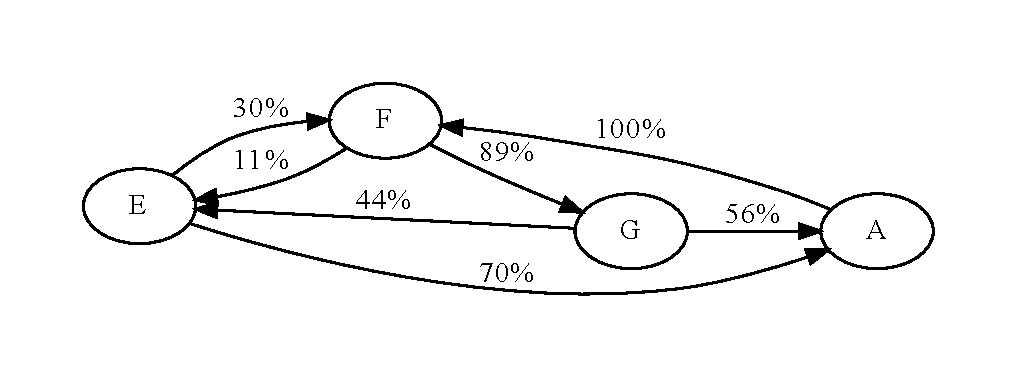
\includegraphics[width=.5\textwidth]{example-graph}
%\caption{Beispielgraph: Die Noten E, F, G und A mit gewissen Wahrscheinlichkeiten verbunden}
\end{figure}

In diesem konkreten Graphen sind die Noten E, F, G und A als Knoten vertreten
(der Einfachheit halber sind die Notenlängen weggelassen). Beispielsweise vom E
führen zwei Kanten weg, eine zum F mit dreißigprozentiger Wahrscheinlichkeit und
eine zum A mit siebzigprozentiger Wahrscheinlichkeit, d. h. nach dem E kommt in
sieben von zehn Fällen das A und in den drei übrigen das F. Analog verhält
es sich mit den anderen Noten.

Diese Darstellung ist in gewisser Weise auch nur eine ausdrucksstärkere Form
einer normalen Notation, denn ein Weg durch den obigen
Graphes könnte so aussehen:

\begin{figure}[h]
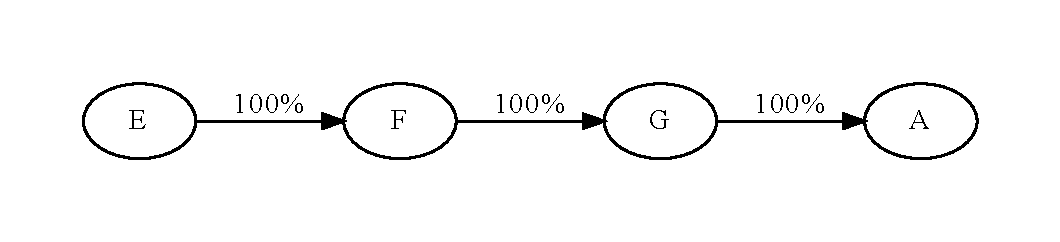
\includegraphics[width=.5\textwidth]{example-graph-interpretation}
\end{figure}

Diese Interpretation, die eine Wahrscheinlichkeit von ca. 15\% hat,
entspricht einer einfachen, linearen Notation, wie sie in einem Gesangsbuch
stehen könnte. Wir sehen also, dass solche probabilistiche Noten (wie unser
Graph von vorhin) durch ein Verfahren, das ich einfach in einer Erweiterung des
Begriffs als Interpretieren bezeichne, auf eine lineare Notation reduziert
werden können, die mit einem Instrument oder vom Computer gespielt werden können. Es
ist sogar nicht nur eine lineare Notation, sondern -- je nach vorgegebenem Graph
-- eine Vielzahl ihrer möglich. Beispielsweise wäre eine weitere:

\begin{figure}[h]
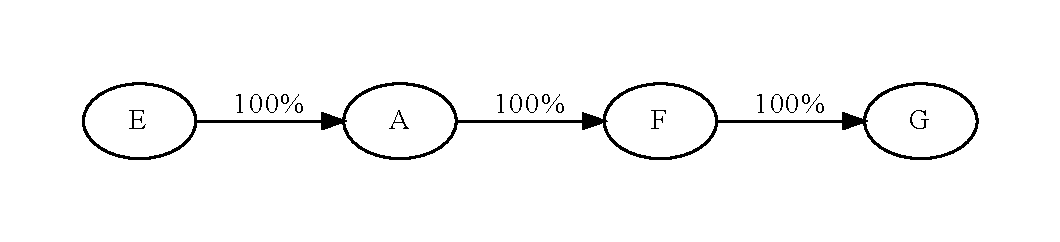
\includegraphics[width=.5\textwidth]{example-graph-interpretation2}
\end{figure}

Ähnlich enthält der ursprüngliche Graph weitere Möglichkeiten von klassischen
Tonabfolgen. Insofern stellt eine probabilistische Notation eine
ausdruckstärkere und mächtigere Notation dar, da sie beliebig viele klassische
fassen kann.

Zu beachten ist bei den beiden
Beispielinterpretationen noch: Sie sind nach vier Noten abgeschnitten, denn, da
von jedem Knoten mindestens eine Kante ausgeht, könnte man den Graphen
potentiell unendlich lang ablaufen und würde somit eine unendlich lange
Interpretation generieren.

Was aus dieser Grundidee zu machen war, schien mir von Anfang an recht klar: Als
Software implementieren, um ein graphisches Interface bereitzustellen, das es
erlaubt, probabilistische Notation zu erstellen, zu editieren und abzuspielen.

\section*{Umsetzung}

Gleich zu Beginn war klar, dass Haskell die Programmiersprache der Wahl werden
sollte. Sie ist die Sprache, die ich in den letzten Jahren am aktivsten
verwendet habe und mir einiges bietet: Statische Typisierung, um Fehler
vorzubeugen, ein expressives Typsystem, das es erlaubt, Daten besser zu
strukturieren, und funktionale Programmierparadigmen, die sich für mich sehr
natürlich anfühlen und das Testen von Programmen erleichtern, um einige Vorzüge zu nennen.

Zunächst konzentrierte ich mich darauf, den Graphen und den
Interpretationsalgorithmus als Bibliothek zu implementieren. In der ersten
Iteration dieser Bibliothek, noch {\it probable music} genannt, begann ich auch
einen eigenen Softwaresynthesizer zu implementieren, der flexibel auf
verschiedenen Plattformen und zu verschiedenen Zwecken verwendet werden kann.
Der Synthesizer konnte jegliche Darstellungen von Klängen, Tönen oder Musik dank
flexibler Architektur in tatsächliche Töne bzw. Audiowellen umwandeln. Dies
ergab interessante Möglichkeiten, sich außerhalb des
Zwölftonsystems zu bewegen. Die Tonerzeugung basierte dann auf einer freien
Monade \cite{free_monad}, die die Instruktionen ›Warten‹ und ›Abspielen‹ kannte.
Indem man diese Instruktionen für verschiedene Audiosystem, wie SDL \cite{sdl},
Jack \cite{jack} oder auch Audiodateien wie WAV \cite{wav} implementierte,
konnte man verschiedene Plattformen unterstützen. Allerdings gestaltete es sich
schwierig, einen gut klingenden Synthesizer zu schreiben, denn die
Messlatte ist im Vergleich zu realen Instrumenten hoch. Hinzu kamen noch einige
Performance-Probleme mit meinem maschinennahen Audio-Code.

Also entschied ich mich, die Library vor allem auf den Graphen und die
dazugehörigen Algorithmen zu fokusieren und zur Tonerzeugung eine geeignete
Abstraktion zu verwenden, um diese zu vereinfachen. Ich habe hierfür MIDI
gewählt, eine Technologie, die schon lang in allen Arten von Software und
Hardware zur Musikproduktion verwendet wird. MIDI basiert auf einer
Abfolge von zeitlich abgestimmten Nachrichten, wie zum Beispiel ›Note C an‹ oder
›Note C aus‹. Aufgrund dieser Nachrichten kann man die Erzeugung und das
Abspielen von Musik zwischen mehreren Programmen aufteilen. Außerdem erlaubt es,
die bereits existierende Infrastruktur für MIDI-Verarbeitung zu verwenden, die
sehr beachtlich ist. Für MIDI verwendet {\it likely music} die
Open-Source-Bibliothek Euterpea\footnote{Ich musste allerdings aufgrund von
Inkompatibilitäten mit den aktuellen Haskell-Paketen diese selbst beheben
\cite{euterpea_fork}. Diese Änderung wartet \cite{euterpea_issue} aktuell (Stand
23.09.2017) darauf, vom Hauptentwickler
in den Code von Euterpea übernommen zu werden.}
\cite{euterpea}, die unter anderem eine kleine Abstraktion über MIDI enthält.
Sie erlaubt es, in einem internen Format Musik zu
konstruieren und anschließend als MIDI zu exportieren bzw. an ein anderes
Programm zur Weiterverarbeitung zu schicken.

Bei der Darstellung des Graphen habe ich mich vor allem darauf konzentriert,
den Interpretationsalgorithmus, also das (zufällige) Ablaufen des Graphen,
möglichst effizient zu gestalten. Da es sich um einen gerichten Graphen handelt,
ist es besonders wichtig zu wissen, wohin man von einem gegebenen Knoten aus
gelangen kann bzw. welche Kanten von einem Knoten weggehen. So gelangt man in unserem Beispiel
aus dem vorherigen Kapitel vom Knoten mit dem E zu den Knoten mit F und
A. Es muss also möglichst effizient sein, die Kanten nachzuschlagen, die von
einem Knoten {\it wegführen}. Mit der Datenstruktur {\it Map} \cite{map} (im
deutschen Sprachgebrauch typischerweise {\it assoziative Datenfeld} bzw. {\it
assoziatives Array}) kann
man genau das sehr leicht realisieren: Man verwendet die Knoten als Schlüssel und
eine Liste von Kanten, die vom Schlüssel weggehen, als Elemente. Wenn
der Algorithmus nun einen Knoten nachschlägt, erhält er direkt die Kanten, die
von diesem Knoten weggehen und somit auch die nächsten möglichen Knoten. Dies
ist die einzige Information, die in jedem Schritt benötigt wird. Die Operation
des Nachschlagen hat in einem {\it Map} die Komplexität $O(\log n)$
\cite{map_lookup}, d. h. die Zeit, die benötigt wird, um ein Element
nachzuschlagen, steigt mit dem Wachsen der Datenstruktur logarithmisch
(d. h. weniger starkes Wachstum als linear!). Damit bleibt auch das Interpretieren
großer Graphen ziemlich schnell. Der Code für die Datenstruktur findet
sich im Abschnitt~\nameref{sec:library}, Zeile 30 bis 43.

Der Interpretationsalgorithmus selbst ist rekursiv \cite{wikipedia_rekursion} gestaltet und findet sich in
der Funktion \lstinline|interpretation|, siehe
Abschnitt~\nameref{sec:library}, Zeile 52 bis 60. Diese Funktion benötigt
einen initialisierten Pseudozufallszahlengenerator
\cite{random_random_gen,wikipedia_prng}, den
zu interpretierenden Graphen in der eben besprochenen Datenstruktur und einen
Startknoten. Nach Ablauf der Berechnung gibt die resultierende Interpretation
im MIDI-Format von Euterpea \cite{euterpea} zurück. Zunächst wird der Startknoten
im Graphen nachgeschlagen, so werden die Kanten bzw. die nächsten möglichen Knoten
erhalten. Nun gibt es zwei Möglichkeiten für den weiteren Verlauf:
\begin{enumerate}
  \item Es gibt keine Kanten, die von diesem Knoten ausgehen. Also wird die
    bisher generierte Interpretation einfach zurückgegeben, die Funktion
    terminiert.
  \item Wenn es eine oder mehr Kanten vom Knoten aus gibt, wird eine (reelle) Zufallszahl
    zwischen $0$ und $1$ berechnet und mittels der Hilfsfunktion \lstinline|edgeForRoll|
    (siehe Abschnitt~\nameref{sec:library}, Zeile 62 - 67) die
    Kante erhalten, die gemäß des zufälligen Ergebnis als nächstes abgelaufen werden
    soll. Nun ergibt sich das gleiche Problem wie zu Beginn der
    Interpretation: Man kennt einen Knoten und will wissen, wie es weitergeht. Also
    wird nach der Ermittlung des zweiten Knotens die MIDI-Nachrichten aus dem
    Startknoten extrahiert und dann der Interpretationsalgorithmus nochmal bzw.
    rekursiv aufgerufen -- nur mit dem Folgeknoten als Startknoten. Dessen
    Ergebnis wird an die aktuellen MIDI-Nachrichten angehängt, was jener Aufruf auch
    seinerseits wieder macht. So entsteht rekursiv eine (potentiell unendliche)
    Verkettung von MIDI-Nachrichten, die letztlich die finale Interpretation ergeben.
\end{enumerate}

Da die meisten Graphen vermutlich vollständig untereinander verbunden sein
werden, wie zum Beispiel der Beispielgraph im ersten Abschnitt, entstehen unendlich
lange Interpretationen. Diese zu erstellen benötigt natürgemäß natürlich auch
unendlich viel Zeit -- der Interpretationsalgorithmus terminiert also nicht.
Die einfache Antwort auf dieses Problem ist die Begrenzung der Länge der
Interpretation auf eine gewisse Anzahl von Noten, was sich dank eines
Sprachfeatures von Haskell -- Lazy Evaluation \cite{wikipedia_laziness} --
leicht umsetzen lässt. Denn mit Lazy Evaluation wird nur das berechnet, was im
Moment benötigt wird. Somit werden zum Beispiel nur die ersten vier benötigten
Noten berechnet und nicht die unendlich vielen die eigentlich noch darauf folgen
würden -- genau dies wird durch die Funktion
\lstinline|takeNotes| (siehe
Abschnitt~\nameref{sec:library}, Zeile 79 - 86) realisiert.

Nun können wir probabilistische Musik in Graphen darstellen, diese automatisch
interpretieren und dank Euterpea nach MIDI exportieren. Was fehlt, ist eine
angenehme Benutzerschnittstelle.

Zur Technologie für die Benutzerschnittstelle gab es für mich folgende
Überlegungen: Zum einen sollte es leicht portabel bzw. auf jedem System laufen
sowie außerdem einen begrenzten Entwicklungsaufwand mit sich bringen, damit es
bis zum Einsendeschluss auch fertig sein würde. Ich selbst entwickle meine Software auf
GNU/Linux, aber zur Abgabe müsste es auf macOS und / oder Windows laufen. Alle
größeren Frameworks für Graphische Interfaces für GNU/Linux, wie zum Beispiel Qt
\cite{qt} oder GTK \cite{gtk}, laufen auch auf den anderen großer
Betriebssystemen. Allerdings bin ich nicht besonders vertraut mit irgendeinem
dieser Frameworks. Außerdem war ich mir nicht sicher, wie stressfrei die
Verwendung dieser von Haskell aus sein würde (denn klassischerweise verwendet
man C oder C++). Also entschied ich mich {\it likely music} als Webapplikation,
die einfach in gängigen Browsern läuft, zu implementieren. Das hat einige
Vorteile für mich, unter anderem, dass es leicht zu testen ist, weil die Browser
eigentlich überall gleich sind, und, dass ich schon einige Erfahrung in
Webentwicklung hatte.

Allerdings hatte ich die Library schon in Haskell implementiert, in Browsern
läuft aber nur JavaScript (ohne größeren Aufwand zumindest). Also musste
ein Programm her, um die Kommunikation zwischen der Library und der
Webapplikation zu realisieren. Ich entschied mich für eine
Client-Server-Architektur \cite{wikipedia_client_server}, also einen Server, der
die Interpretation und den Export von Sounddateien für den Client, also die
Webapplikation, übernimmt. Der Client wiederum müsste sich ausschließlich um ein
ansprechendes Interface kümmern. Die ungefähre Gesamtarchitektur sieht also nun
so aus:

\begin{figure}[h]
  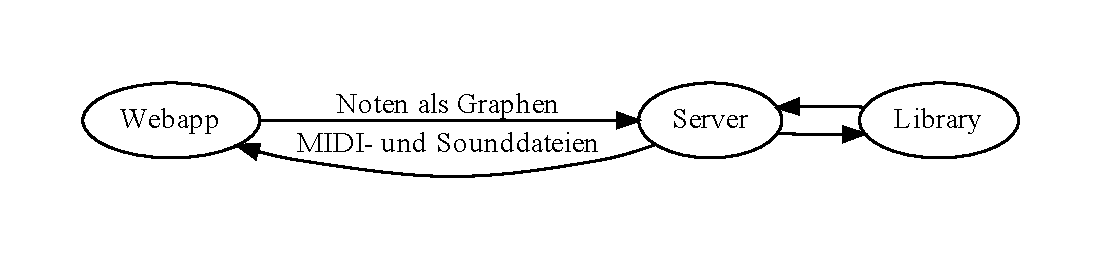
\includegraphics[width=0.5\textwidth]{architektur}
\end{figure}

Der Server basiert auf den Libraries servant \cite{servant} als Webframework.
Wie im Abschnitt~\nameref{sec:backend} zu sehen, besteht das Serverbackend aus
zwei Dateien Quelltext: In \lstinline|Api.hs| wird die
Struktur der REST-API \cite{wikipedia_rest} definiert, mittels der die
Webapplikation mit dem Server kommuniziert. Der Server bietet folgende Funktionalität
an:

\begin{itemize}
  \item \lstinline|/interpretation/mid| An diesen Endpunkt
    schickt die Webapplikation einen Graphen plus einiger Parameter in Form von JSON
    \cite{json} und erhält eine Interpretation auf Basis des Algorithmus als
    MIDI-Datei zurück.
  \item \lstinline|/interpretation/wav| Gleich wie der
    obige Endpunkt, allerdings wird vorher
    noch das MIDI mittels des MIDI-Synthesizers fluidsynth \cite{fluidsynth}
    in eine WAV-Datei konvertiert, so dass man die Interpretation direkt anhören kann.
  \item Außerdem liefert der Server die statischen Dateien der Webapplikation, wie das
    nötige HTML, JavaScript und CSS.
\end{itemize}

Die erwähnten Parameter sind nur folgende drei:

\begin{itemize}
  \item Der Anfangsknoten der Interpretation im Graphen,
    den der Algorithmus benötigt (wie oben besprochen).
  \item Die Länge der Interpretation als die maximale Anzahl an Noten in der
    Interpretation.
  \item Der Startwert für den Pseudozufallszahlengenerator
    \cite{wikipedia_prng}, der für die Interpretation verwendet werden soll.
    Da derselbe Startwert in die selbe Interpretation resultiert, erlaubt dies,
    sich interessante Interpretationen zu merken und zum Beispiel zu einer
    Interpretation noch die MIDI-Version zusätzlich herunterzuladen.
\end{itemize}

Dies ist auch schon alles, was das Serverbackend tut, denn es ist nur als
minimaler Aufsatz auf die Library konzipiert. Das meiste für Benutzer*innen relevante
passiert in der Webapplikation, die folgendermaßen aussieht:

\begin{figure}[h]
  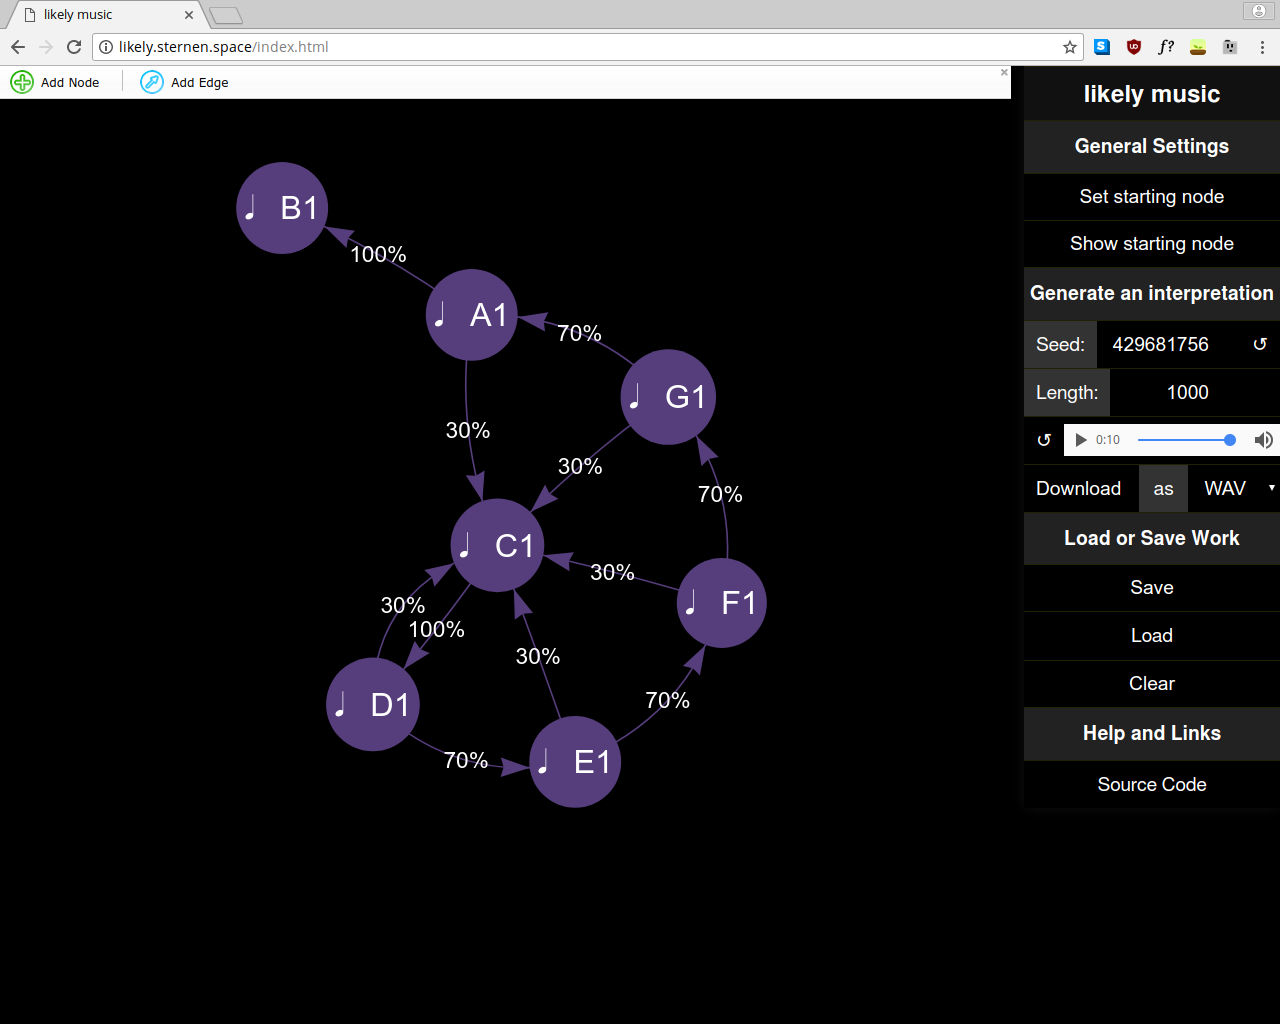
\includegraphics[width=.5\textwidth]{screenshots/start.png}
\end{figure}

Den Kern der Applikation bildet der Grapheditor links, der auf der Library
vis.js\footnote{Eigentlich nur ein Teil von vis.js namens {\it network}
\cite{visjs_network}, aber
ich werde vis.js immer der Kürze halber synonym für {\it vis.js network} verwenden.}
\cite{visjs} basiert. vis.js kümmert sich um einen sehr gut anpassbaren
Grapheneditoren, in dem der*die Benutzer*in Knoten und Kanten hinzufügen, löschen und
ändern kann. Da die Library Callbacks \cite{wikipedia_callback} bereitstellt,
ist es leicht den Rest der Applikation mit dem Editor zu integrieren.

Wenn ein Knoten oder eine Kante geändert wird, wird diese Änderung in eine
Zustandsvariable
der Applikation mitübernommen und die Zusatzinformationen der Knoten und
Kanten, also Notenlänge und Tonhöhe (Knoten) bzw. Wahrscheinlichkeit (Kante),
von dem*der Benutzer*in in einer Einblendung abgefragt und ebenfalls
abgespeichert. So gelingt es, den
Grapheditor so zu integrieren, dass der Graph zur Kommunikation mit dem Server
und sonstiger Verarbeitung zur Verfügung steht. Die doppelte Speicherung der
reinen Graphdaten kommt daher, dass
vis.js es leider nicht erlaubt, die bereits im Editor vorhandenen Daten
abzufragen, daher büßt die Architektur der Applikation leider ein wenig
an Eleganz ein.

In der Seitenspalte passiert dann alles, was relevant für die Verarbeitung der
links entstehenden Notation ist. Zum einen kann der Notationsgraph abgespeichert
oder ein gespeicherter geöffnet werden, zum anderen ist es möglich,
Interpretationen generieren zu lassen, diese direkt im Browser abzuspielen oder
als MIDI oder WAV herunterzuladen. Die Seitenspalte ist im folgenden abgebildet.

\begin{wrapfigure}{r}{.3\textwidth}
  \begin{center}
    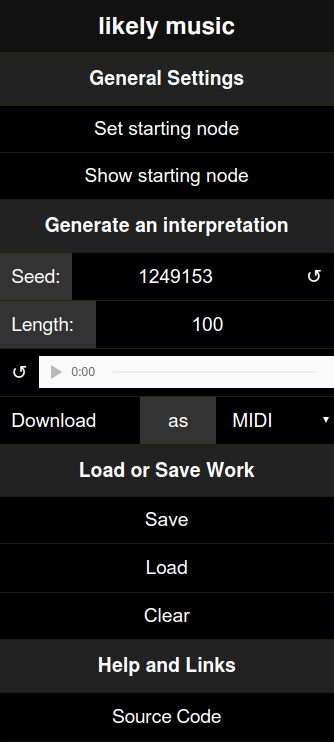
\includegraphics[width=.25\textwidth]{screenshots/sidebar}
  \end{center}
\end{wrapfigure}

Das Speichern und Öffnen von Notationen basiert auf JSON-Dateien
\cite{json} in bestimmten Format, die als
\lstinline|<dateiname>.score.json| abgespeichert werden.
Eine solche enthält eine Liste aller Knoten plus Zusatzinformationen und eine
Liste aller Kanten plus Zusatzinformationen. Wie eine solche aussehen kann,
sieht man im Abschnitt~\nameref{sec:web} (letzte Datei). Genau dieses Format
wird übrigens auch zur Kommunikation mit dem Server verwendet, da es den Graphen
verlustlos beschreiben kann.

Der Rest der Applikation kümmert sich vor allem um Interpretation und Export
dieser. Oben in der Seitenleiste kann man die drei erwähnten Parameter setzen.
Der Startknoten wird über markieren dessen im Editor und klicken des
entsprechenden Buttons gesetzt und kann durch Hervorhebung im Graphen auch
angezeigt werden. Der Startwert kann manuell eingegeben (etwa, wenn man
sich einen besonderen notiert hat) oder ein zufälliger durch Verwendung des
Buttons neben dem Feld verwendet werden. Die maximale Interpretationslänge ist
dann darunter und wird ganz unspektakulär eingegeben.

Darunter befindet sich ein Audioplayer, mit dem erstellte Interpretationen
direkt im Browser angehört werden können. Wenn man den Aktualisierungsbutton
links betätigt, nimmt die Applikation alle Parameter sowie den aktuellen Graphen
und sendet mithilfe der JavaScript Fetch API \cite{fetch_api} den Graphen
mitsamt der Parameter an den bereits erwähnten Endpunkt
\lstinline|/interpretation/wav|. Nach diesem Vorgang, der merklich Zeit benötigt,
da fluidsynth \cite{fluidsynth} erst das WAV generieren muss, wird die
Audiodatei in den Player geladen und kann direkt angehört werden.

Gleich unter dem Player kann man die Interpretation als MIDI oder WAV
herunterladen. Dazu wählt man rechts eines der beiden Formate aus und klickt
links auf „Download“. Intern funktioniert dies genau gleich wie der Player, bloß
dass die jeweils der Endpunkte für das entsprechende Format verwendet wird und
die Datei dann direkt heruntergeladen wird statt im Browser weiterverwendet
wird.

Des weiteren werden der aktuelle Graph und die Parameter regelmäßig mittels
LocalStorage \cite{localstorage} zwischengespeichert, die beim Öffnen der
Webapplikation abgefragt wird. So ist gleich der letzte Stand vom letzten mal
geladen und man kann direkt weiterarbeiten.

\subsection*{Lizenzierung}

Der gesamte Quelltext von {\it likely music} ist unter der
{\it GNU Affero General Public License Version 3} lizenziert. Die AGPL ist eine
Freie-Software-Lizenz \cite{gnu_free_software}, das heißt, sie sichert dem*der
Benutzer*in gegenüber dem Entwickler verschiedene Rechte (typischerweise nennt man
vier) zu. Diese Rechte haben alle emanzipatorischen Charakter für den Nutzer:
Das Recht die Software so auszuführen, wie der Nutzer es mag, natürlich
offensichtlichlerweise. Das Recht, den Quellcode zu erhalten und zu untersuchen
hilft vor allem dem*der Benutzer*in zu verstehen, was eigentlich auf
seinem*ihrem Computer vor sich geht, und kann auch der Weiterbildung dienen. Die
Freiheit, die Software frei und ohne Lizenzgebühren an andere weiterzugeben, ist
mir besonders wichtig. Aufgrund diesen Umstandes kann freie Software
unentgeltlich an jede*n weitergegeben werden, was Zugang zu Software unabhängig
des eigenen Geldbeutels erlaubt -- vorausgesetzt man besitzt einen Computer.
Diese Freiheit geht sogar noch weiter, dahingehend, dass auch die Modifikation
ausdrücklich erlaubt (und erwünscht) ist. Somit kann nicht nur jede*r freie
Software erhalten, sondern auch mitgestalten und verbessern. Auch andere freie
Software kann profitieren, indem sie von anderen Projekten Code übernimmt. Dank
der restriktiven Weitergabeklauseln kann aber nie freie Software verwendet oder
verändert werden, ohne dass sie wieder freie Software wird. Freie Software
erhält sozusagen ihre eigene Freiheit.

Mir ist dies an dieser Stelle ein besonderes Anliegen, weil ich -- mit
Sicherheit im Gegensatz zu den allermeisten anderen Wettbewerbteilnehmer*innen
-- mein Projekt komplett mit freier Software erstellen konnte. Ich war nicht auf
eine von drei teuren Softwarelösungen großer Konzerne angewiesen, um meinen
Beitrag anzufertigen, wie das zum Beispiel im Bereich Videoschnitt der Fall ist
(auch weil es kaum ausgereifte freie Software in dem Bereich gibt).

Insofern sehe ich auch den emanzipatorischen Charakter von freier Software, denn
Zugang zu Computern ist größtenteils auch dank von Bibliotheken
selbstverständlich geworden, Zugang zu Software, die mehrere hundert Euro
kostet, aber mit Sicherheit nicht. Der Preis von Software, die ein Konzern
vielleicht auch irgendwann verwahrlosen lässt, ist sicher für viele eine Hürde,
vielleicht sogar eine Hürde an diesem Wettbewerb teilzunehmen.

\section*{Zukünftige Weiterentwicklung}

{\it likely music} als fertig zu bezeichnen wäre nicht ganz falsch und nicht
ganz richtig. Es handelt sich zwar um eine voll funktionsfähige Software, aber
dennoch ist noch einige Weiterentwicklung, für die ich keine Zeit mehr hatte,
denkbar. Folgende Gedanken hatte ich
bisher:

\begin{itemize}
  \item {\bf Unterstützung für Akkorde im Interface.} Zwar unterstützen Euterpea
    und die Library beide Akkorde, aber im Frontend gibt es keine Möglichkeit,
    solche hinzuzufügen, da ich die Euterpea-MIDI-Datenstruktur nicht
    vollständig in JavaScript nachgebaut habe. Dies zu beheben wäre für die
    Zukunft auf jeden Fall wünschenswert.
  \item {\bf Mehrstimmige bzw. parallele probabilistische Musik.} Denkbar wäre
    es, eine Möglichkeit hinzuzufügen mehrere Startknoten auszuwählen, von denen
    dann zwei gleichzeitige Pfade durch den Graph ausgingen. Dies scheint mir
    die interessantes Möglichkeit zu sein, Mehrstimmig für {\it likely music}
    umzusetzen.
  \item {\bf Import bereits durchkomponierter Musik.} Indem man die Möglichkeit
    schafft, bereits in
    konventionellen Notationsprogrammen erstellte Musik zu importieren, könnte man
    ein für den*die Benutzer*in angenehme Möglichkeit bieten, konventionell
    notierter Musik ein probabilistisches Element zu geben bzw. sie
    probabilistisch umzusetzen.
\end{itemize}

Diese Änderungen stehen nicht im Konflikt mit dem bisherigen Grundkonzept und -aufbau von
{\it likely music}, dürften daher ohne größere Probleme umgesetzt werden können.

\section*{Links}

\begin{itemize}
\item Der gesamte Quelltext \url{https://github.com/sternenseemann/likely-music}
\item Eine laufende Instanz\footnote{{\it likely music} ist bisher noch nicht
  auf Performance optimiert worden. Ich glaube nicht, dass genannte Server einen
    größeren Ansturm vor allem wegen des Exports zu WAV (fluidsynth
    \cite{fluidsynth} ist ziemlich
    langsam) aushalten würde. Daher möchte ich darum bitten, diesen Link nicht
    zu veröffentlichen, sondern, falls etwas in der Art gewünscht sein sollte,
    mit mir Rücksprache zu halten.} von {\it likely music} \url{https://likely.sternen.space}
\end{itemize}

\section*{Danksagung}

\begin{itemize}
  \item Meinem Lehrer Bastian Walcher für seine Betreung meines Projekt und derer
    meiner Mitschüler*innen.
  \item Lukas G. für sein Korrekturlesen.
  \item Christine S. für ihr Korrekturlesen.
  \item kohlrabi dafür, dass er sich mit mir über Musikprogrammierung und
    -theorie unterhielt und Ideen zu meinem Projekt beisteuerte.
  \item all dafür, dass er mich in Richtung Musikprogrammierung stieß.
\end{itemize}

\begin{thebibliography}{9}
\bibitem{wikipedia_demoscene}
  \url{https://de.wikipedia.org/wiki/Demoszene}

\bibitem{free_monad}
  \url{http://www.haskellforall.com/2012/07/purify-code-using-free-monads.html}

\bibitem{jack}
  \url{http://www.jackaudio.org/}

\bibitem{sdl}
  \url{https://www.libsdl.org/index.php}

\bibitem{wav}
  \url{https://de.wikipedia.org/wiki/RIFF_WAVE}

\bibitem{midi}
  \url{https://www.midi.org/}

\bibitem{wikipedia_midi}
  \url{https://de.wikipedia.org/wiki/Musical_Instrument_Digital_Interface}

\bibitem{euterpea}
  \url{https://hackage.haskell.org/package/Euterpea}

\bibitem{euterpea_fork}
  \url{https://github.com/sternenseemann/Euterpea2}

\bibitem{euterpea_issue}
  \url{https://github.com/Euterpea/Euterpea2/issues/16}

\bibitem{map}
  \url{https://hackage.haskell.org/package/containers-0.5.10.2/docs/Data-Map-Lazy.html#t:Map}

\bibitem{map_lookup}
  \url{https://hackage.haskell.org/package/containers-0.5.10.2/docs/Data-Map-Lazy.html#v:lookup}

\bibitem{random_random_gen}
  \url{https://hackage.haskell.org/package/random-1.1/docs/System-Random.html#t:RandomGen}

\bibitem{wikipedia_prng}
  \url{https://en.wikipedia.org/wiki/Pseudorandom_number_generator}

\bibitem{wikipedia_rekursion}
  \url{https://de.wikipedia.org/wiki/Rekursion}

\bibitem{wikipedia_laziness}
  \url{https://de.wikipedia.org/wiki/Lazy_Evaluation}

\bibitem{wikipedia_client_server}
  \url{https://en.wikipedia.org/wiki/Client%E2%80%93server_model}

\bibitem{servant}
  \url{https://hackage.haskell.org/package/servant}

\bibitem{wikipedia_rest}
  \url{https://de.wikipedia.org/wiki/Representational_State_Transfer}

\bibitem{json}
  \url{http://json.org/}

\bibitem{qt}
  \url{https://www.qt.io/}

\bibitem{gtk}
  \url{https://www.gtk.org/}

\bibitem{fluidsynth}
  \url{http://www.fluidsynth.org/}

\bibitem{visjs}
  \url{http://visjs.org/}

\bibitem{visjs_network}
  \url{visjs.org/docs/network/}

\bibitem{wikipedia_callback}
  \url{https://en.wikipedia.org/wiki/Callback_(computer_programming)}

\bibitem{fetch_api}
  \url{https://developer.mozilla.org/en-US/docs/Web/API/Fetch_API}

\bibitem{localstorage}
  \url{https://developer.mozilla.org/en-US/docs/Web/API/Web_Storage_API}

\bibitem{agpl}
  \url{https://www.gnu.org/licenses/agpl-3.0.html}

\bibitem{gnu_free_software}
  \url{https://www.gnu.org/philosophy/free-sw.de.html}
\end{thebibliography}

\clearpage
\onecolumn

\section*{Anhang}

\subsection*{Screenshots}
\begin{figure}[H]
  \begin{center}
  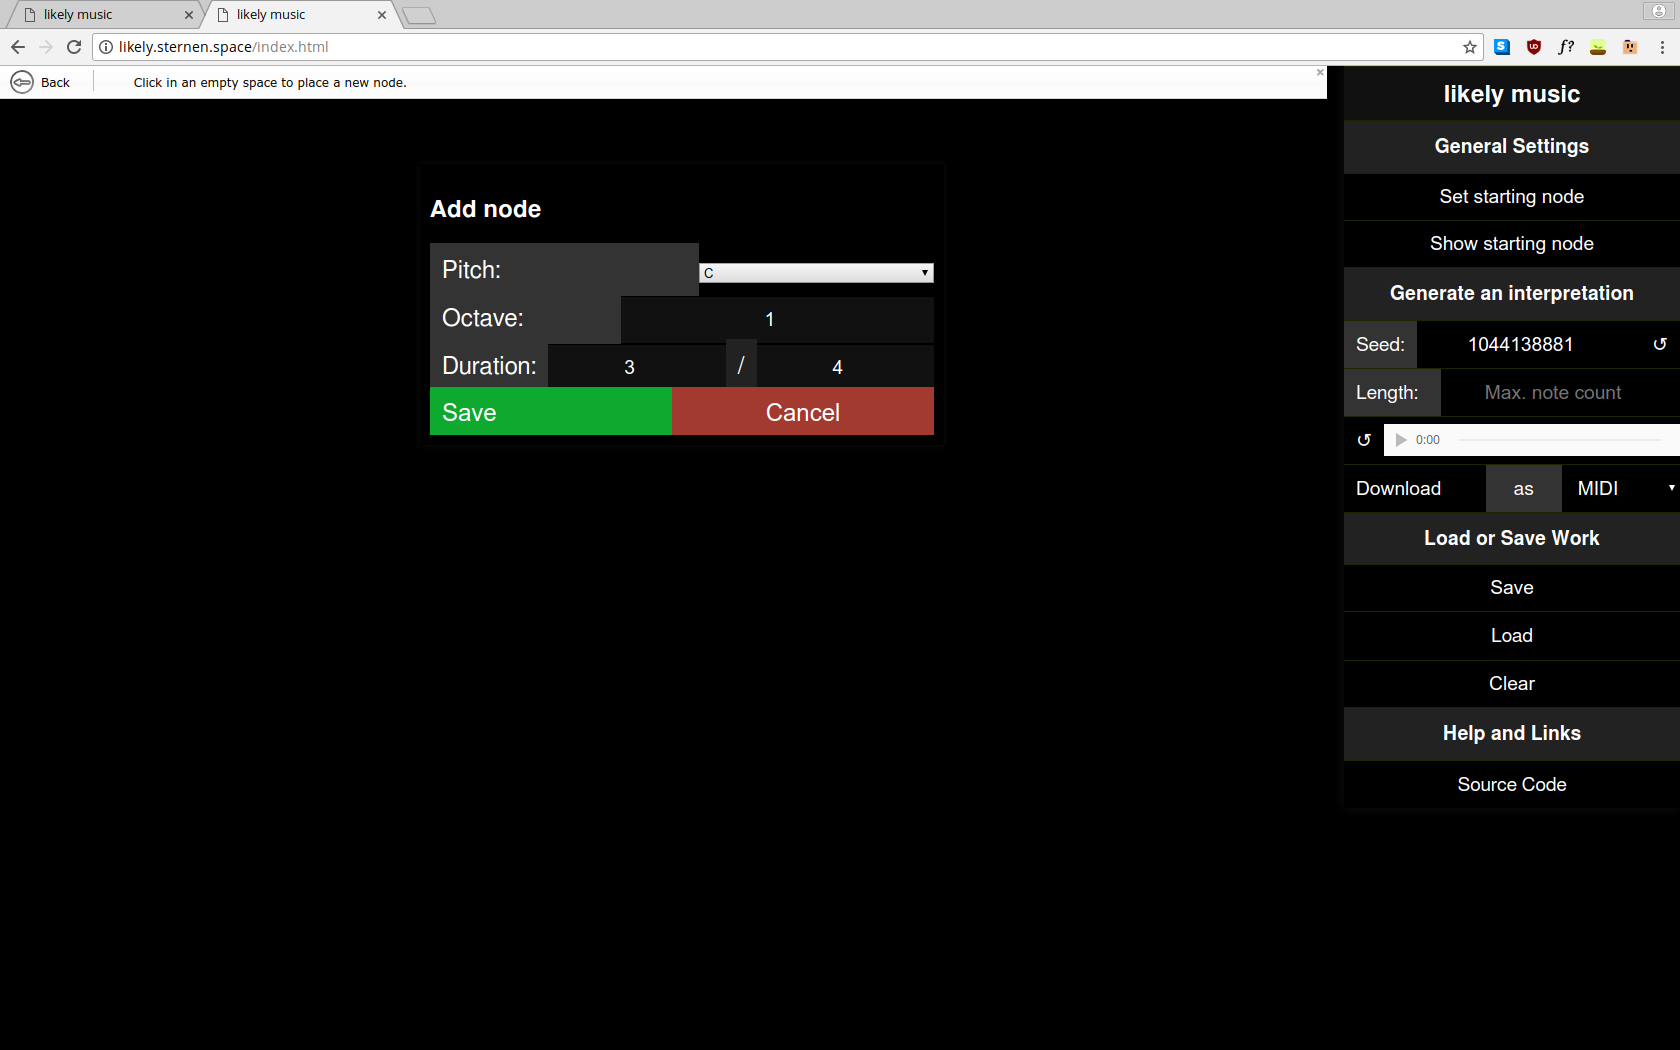
\includegraphics[width=.7\textwidth]{screenshots/add-node.png}
  \end{center}
  \caption{Hinzufügen eines Knotens}
\end{figure}

\begin{figure}[H]
  \begin{center}
  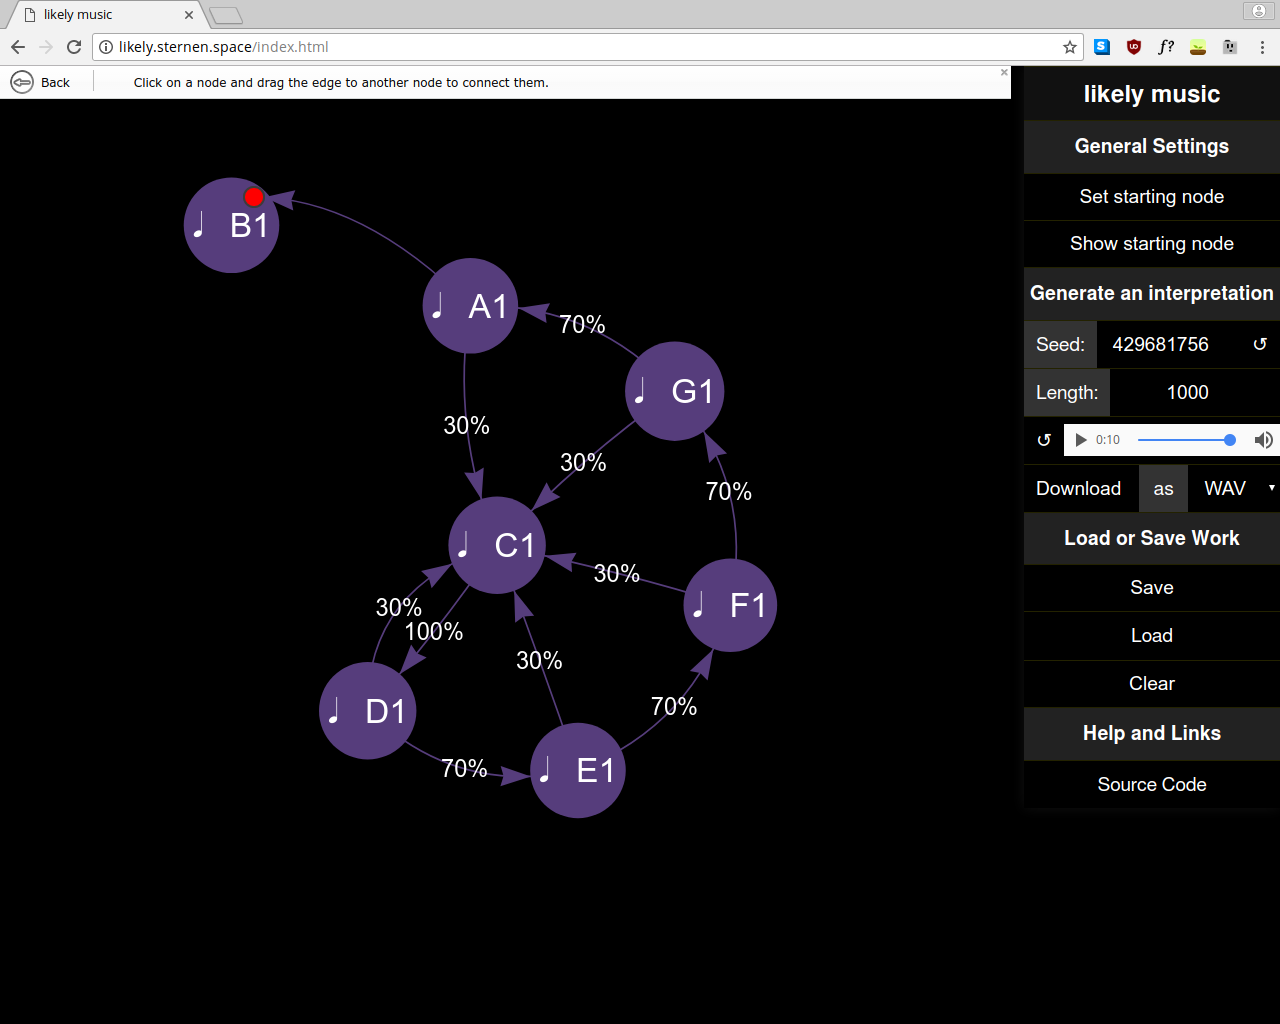
\includegraphics[width=.7\textwidth]{screenshots/add-edge-drag.png}
  \end{center}
  \caption{Verbinden zweier Knoten mit einer Kante}
\end{figure}

\begin{figure}[H]
  \begin{center}
  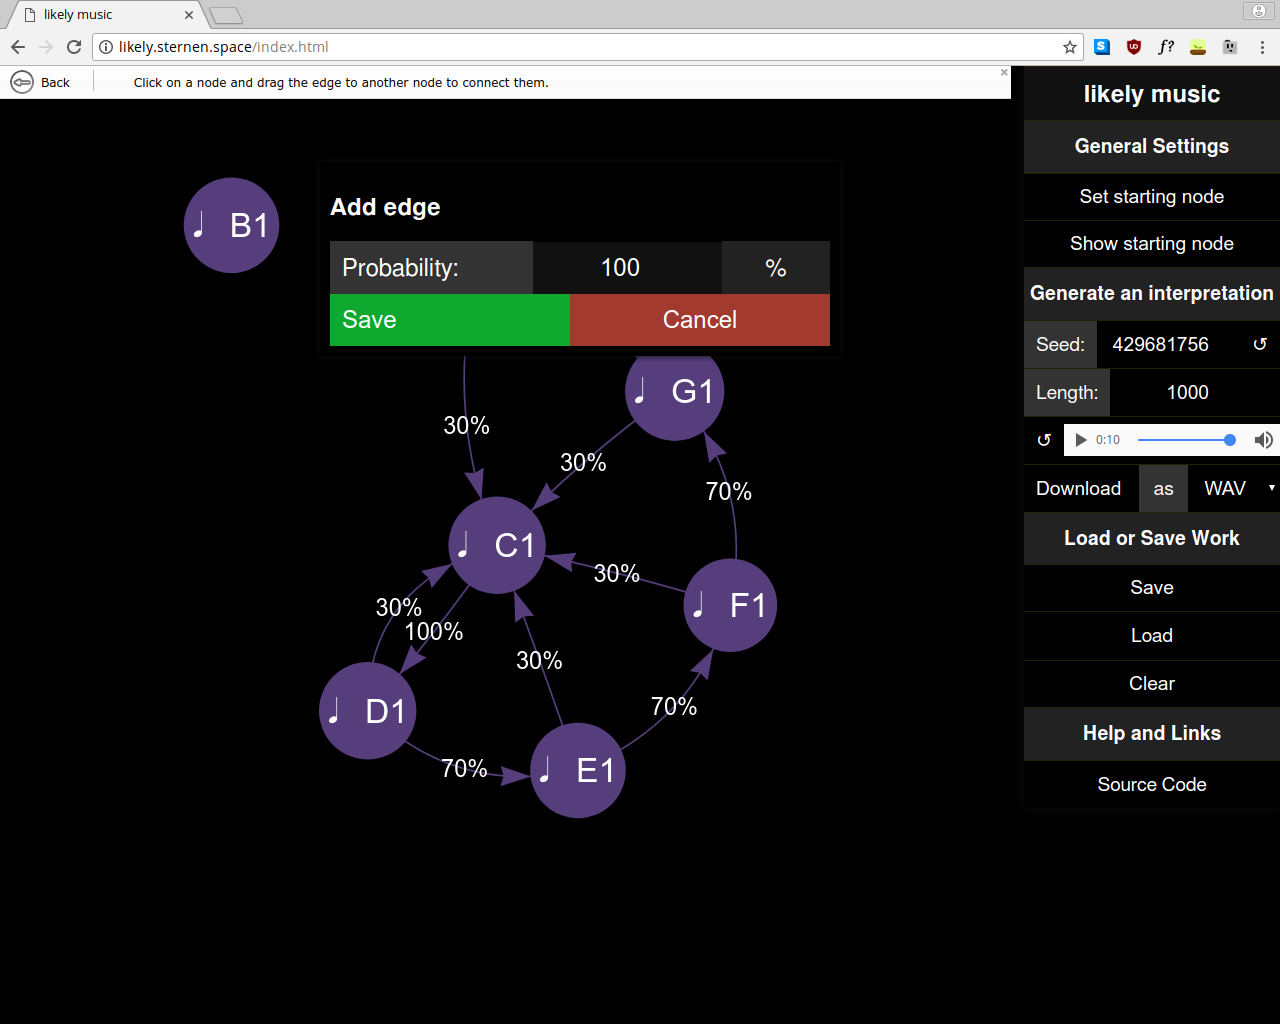
\includegraphics[width=.7\textwidth]{screenshots/add-edge.png}
  \end{center}
  \caption{Setzen der Kanteneigenschaften}
\end{figure}

\begin{figure}[H]
  \begin{center}
  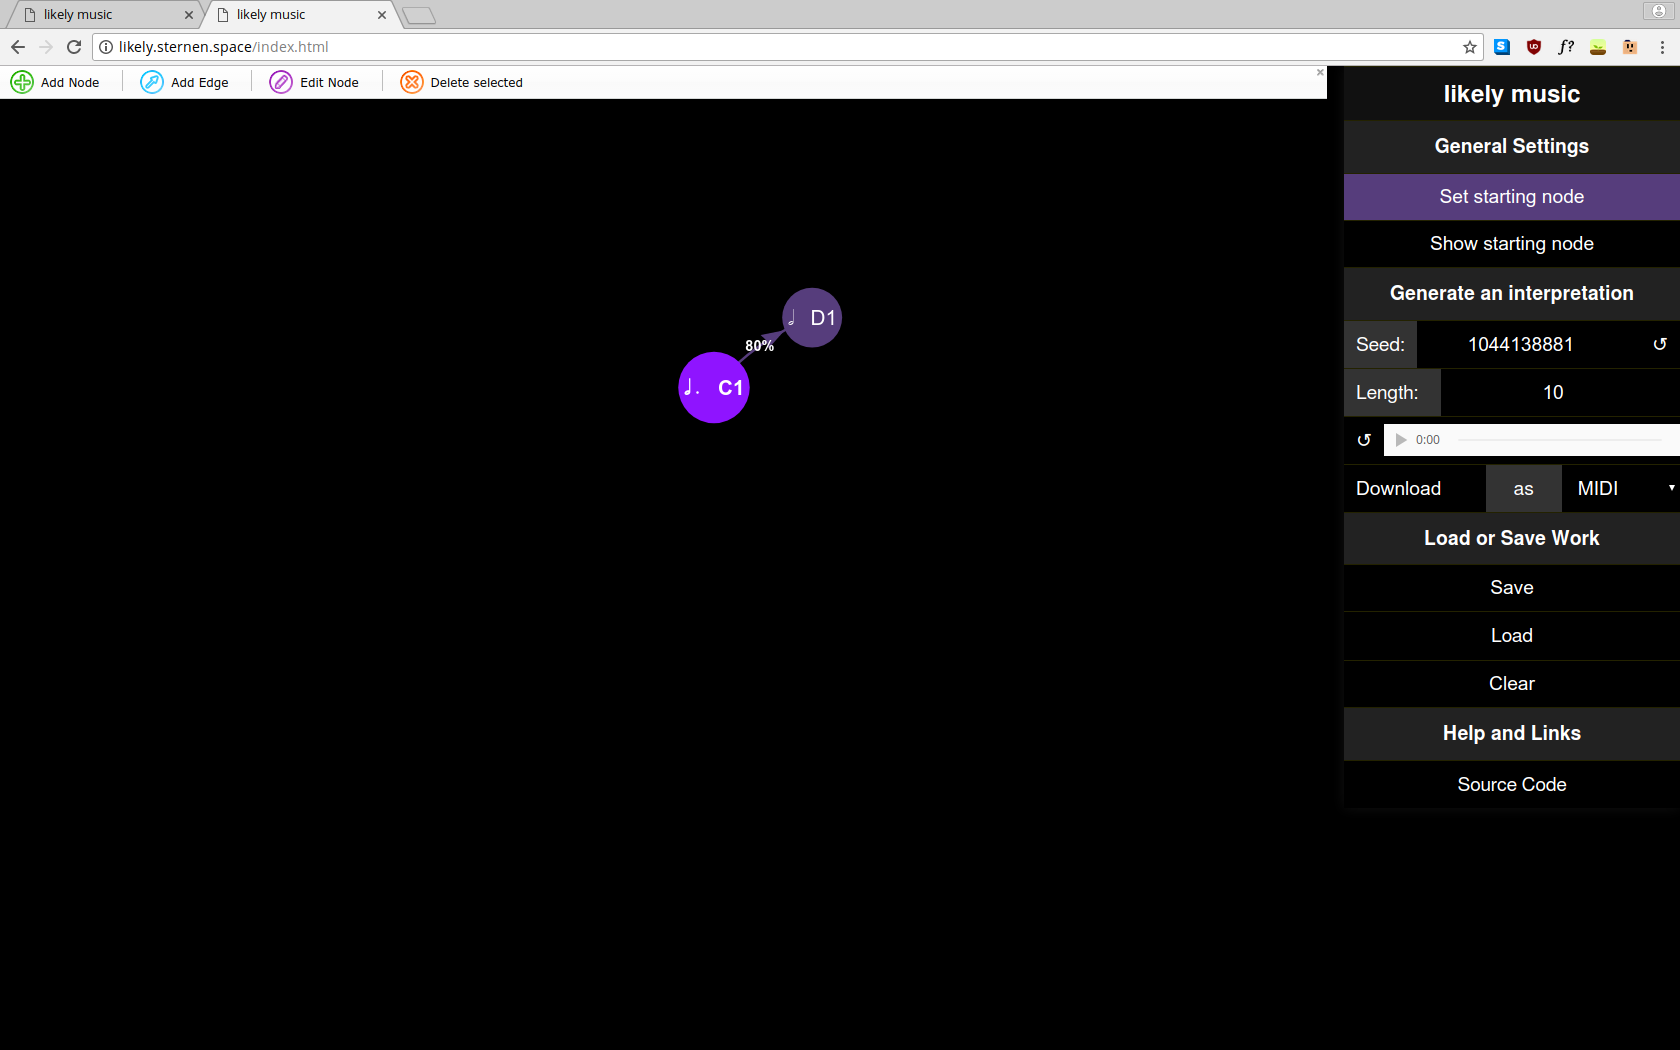
\includegraphics[width=.7\textwidth]{screenshots/starting-node.png}
  \end{center}
  \caption{Setzen des Startknoten durch Auswählen des Knotens}
\end{figure}

\begin{figure}[H]
  \begin{center}
  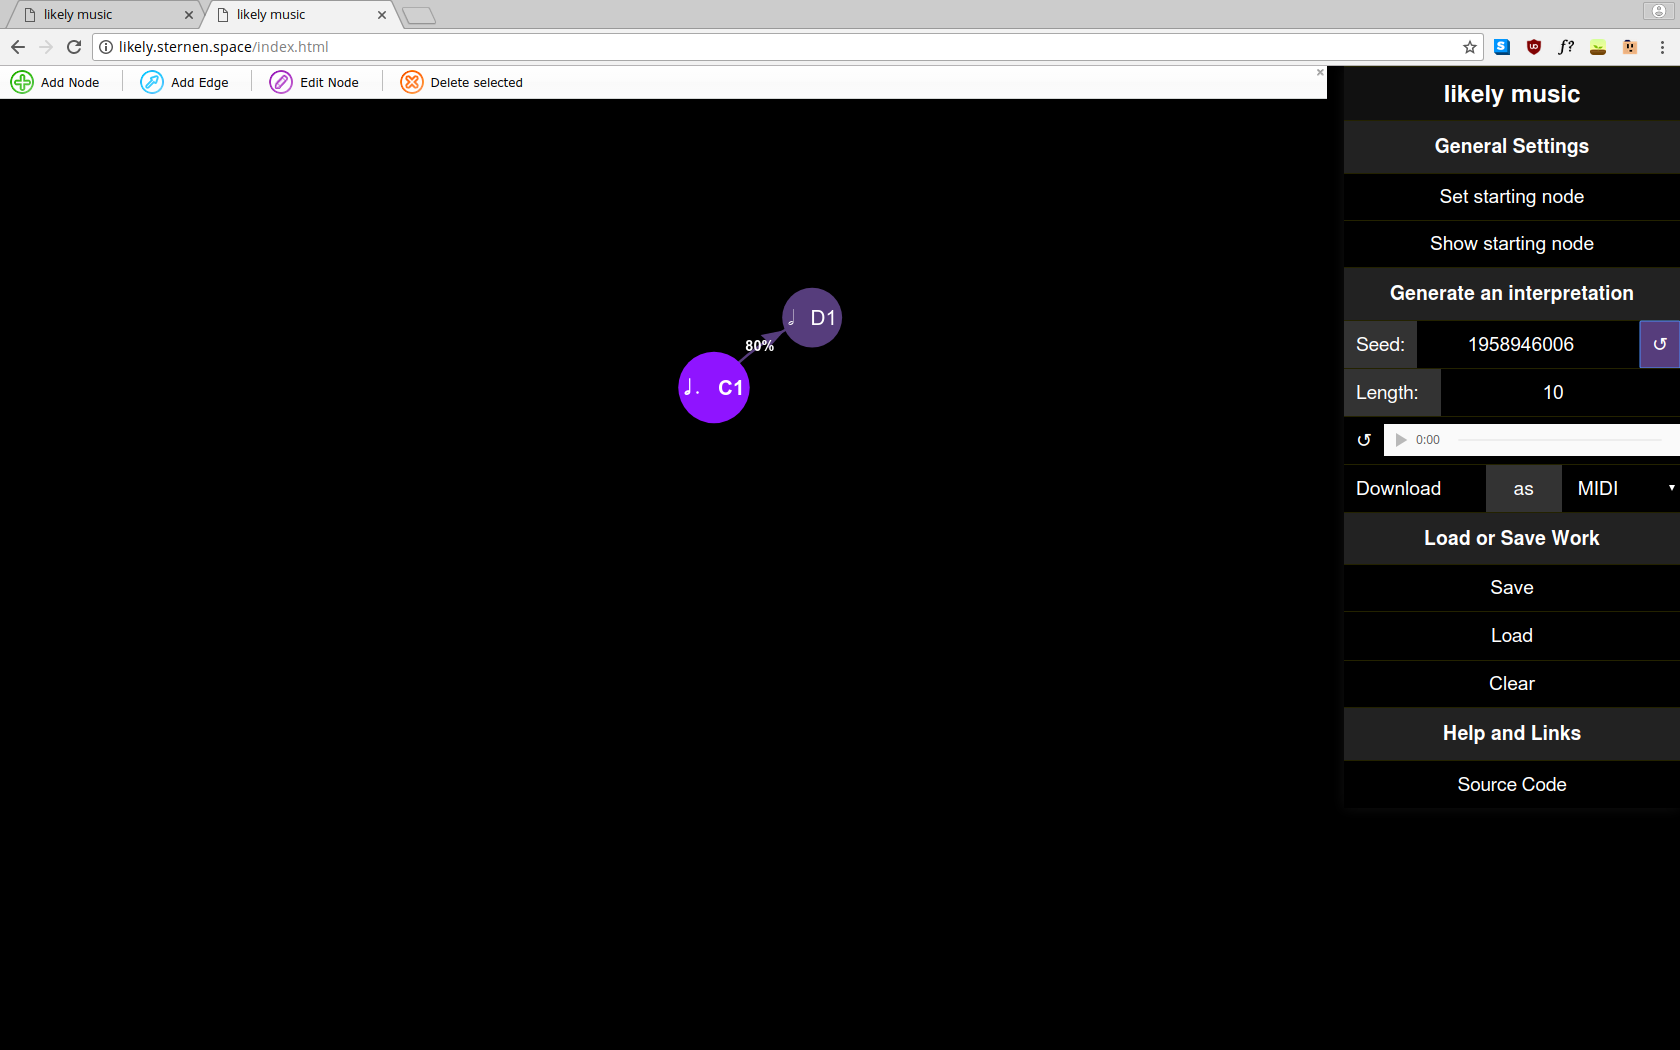
\includegraphics[width=.7\textwidth]{screenshots/new-seed.png}
  \end{center}
  \caption{Auswürfeln eines neuen Startwerts per Knopfdruck}
\end{figure}

\begin{figure}[H]
  \begin{center}
  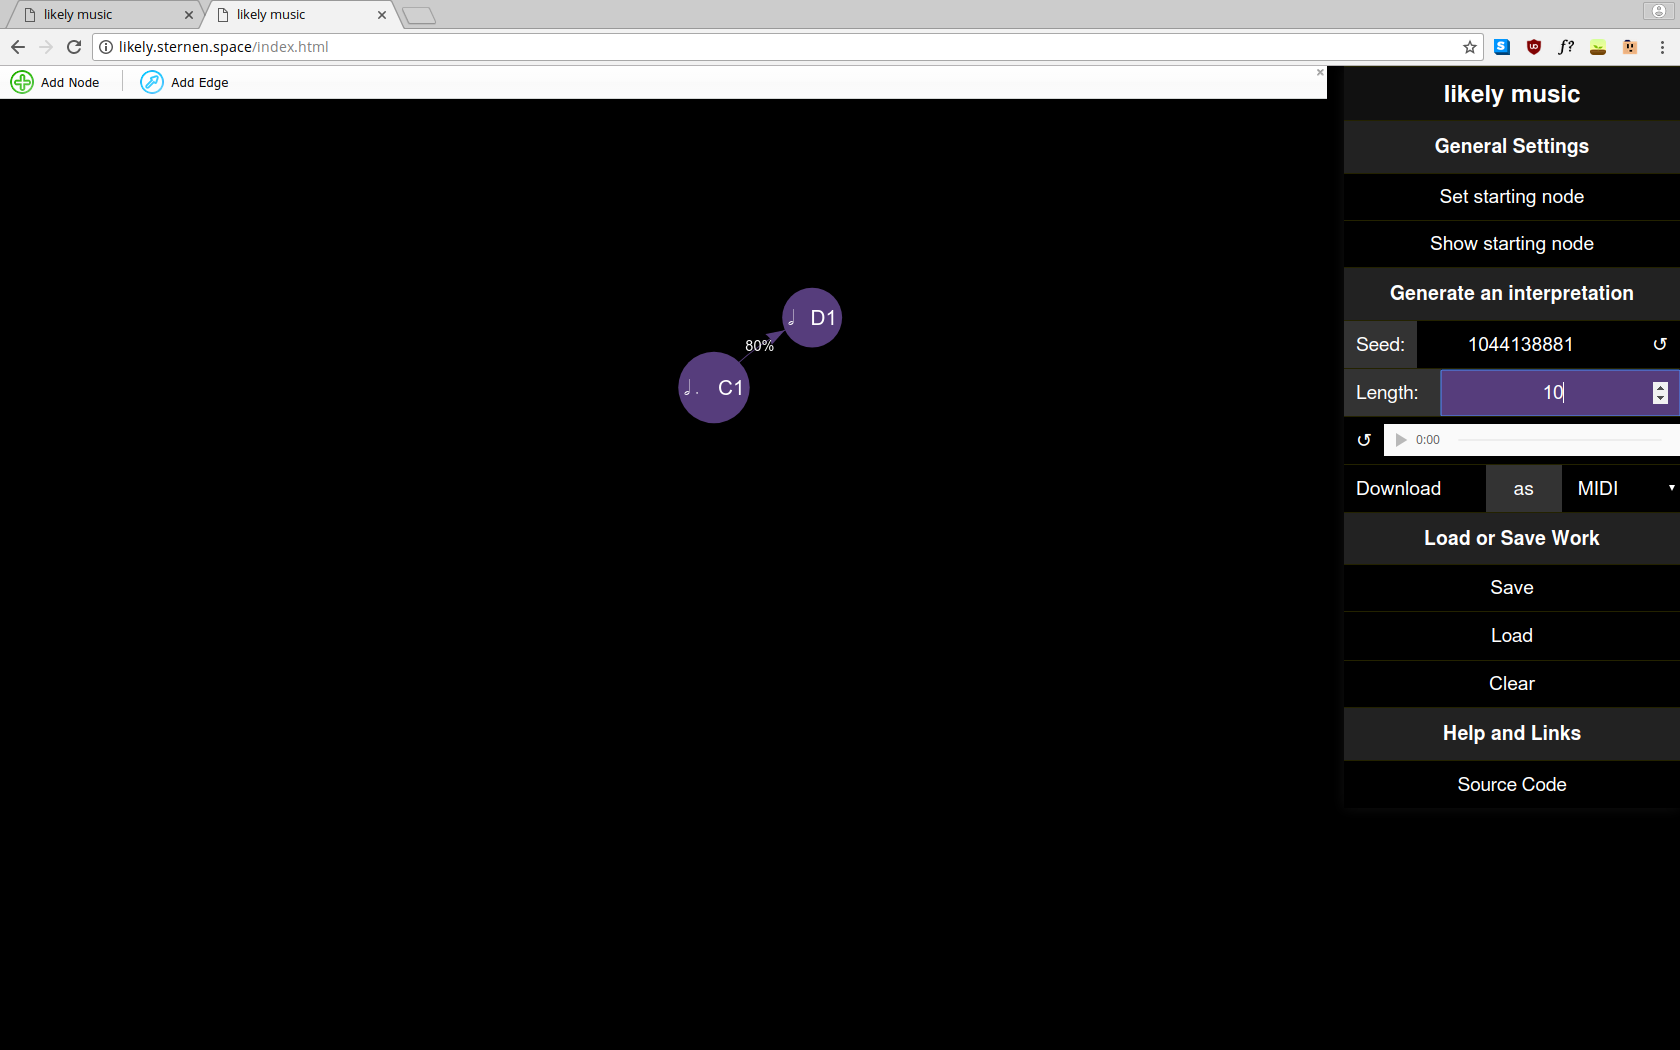
\includegraphics[width=.7\textwidth]{screenshots/length.png}
  \end{center}
  \caption{Setzen der maximalen Interpretationslänge}
\end{figure}

\begin{figure}[H]
  \begin{center}
  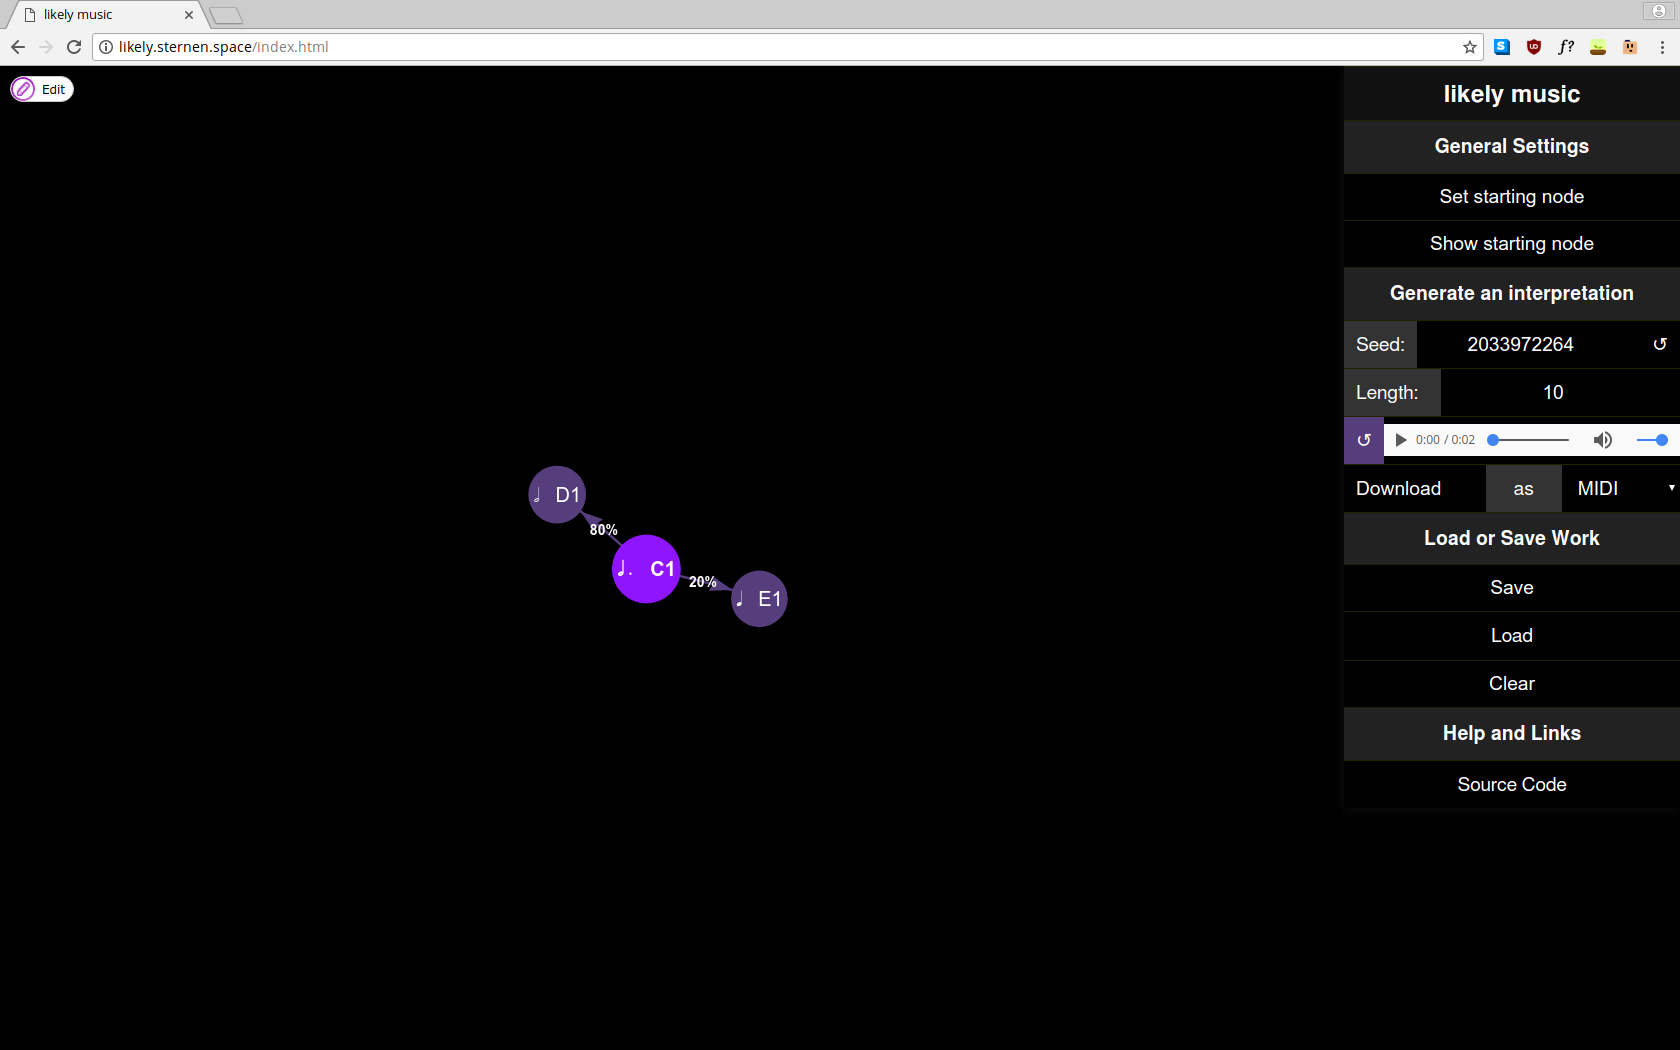
\includegraphics[width=.7\textwidth]{screenshots/reload-player.png}
  \end{center}
  \caption{Laden der Interpretation in den Player}
\end{figure}

\begin{figure}[H]
  \begin{center}
  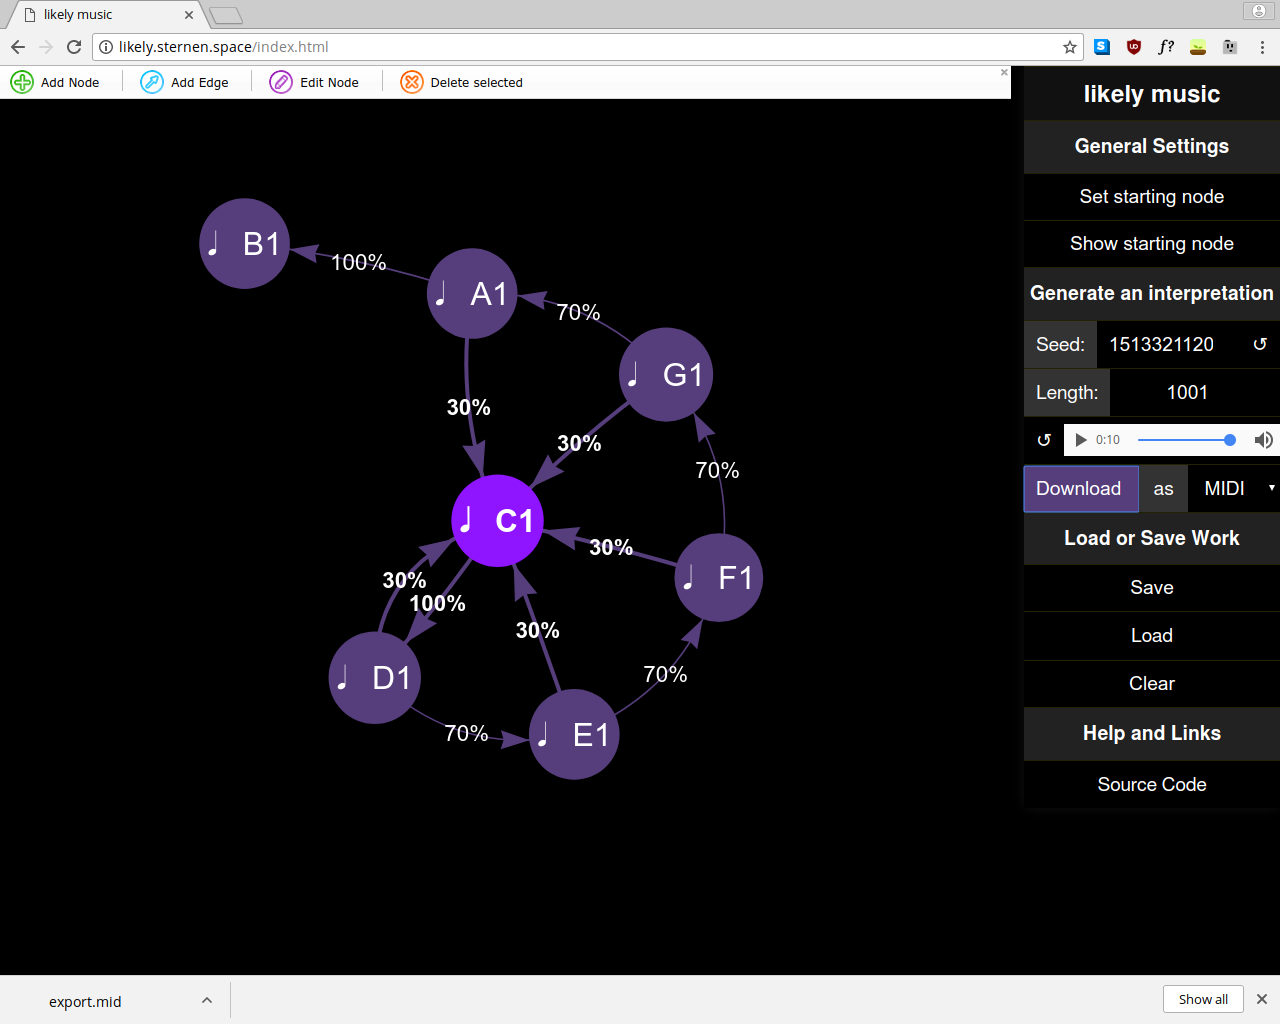
\includegraphics[width=.7\textwidth]{screenshots/download-midi.png}
  \end{center}
  \caption{Download der Interpretation als MIDI-Datei}
\end{figure}

\begin{figure}[H]
  \begin{center}
  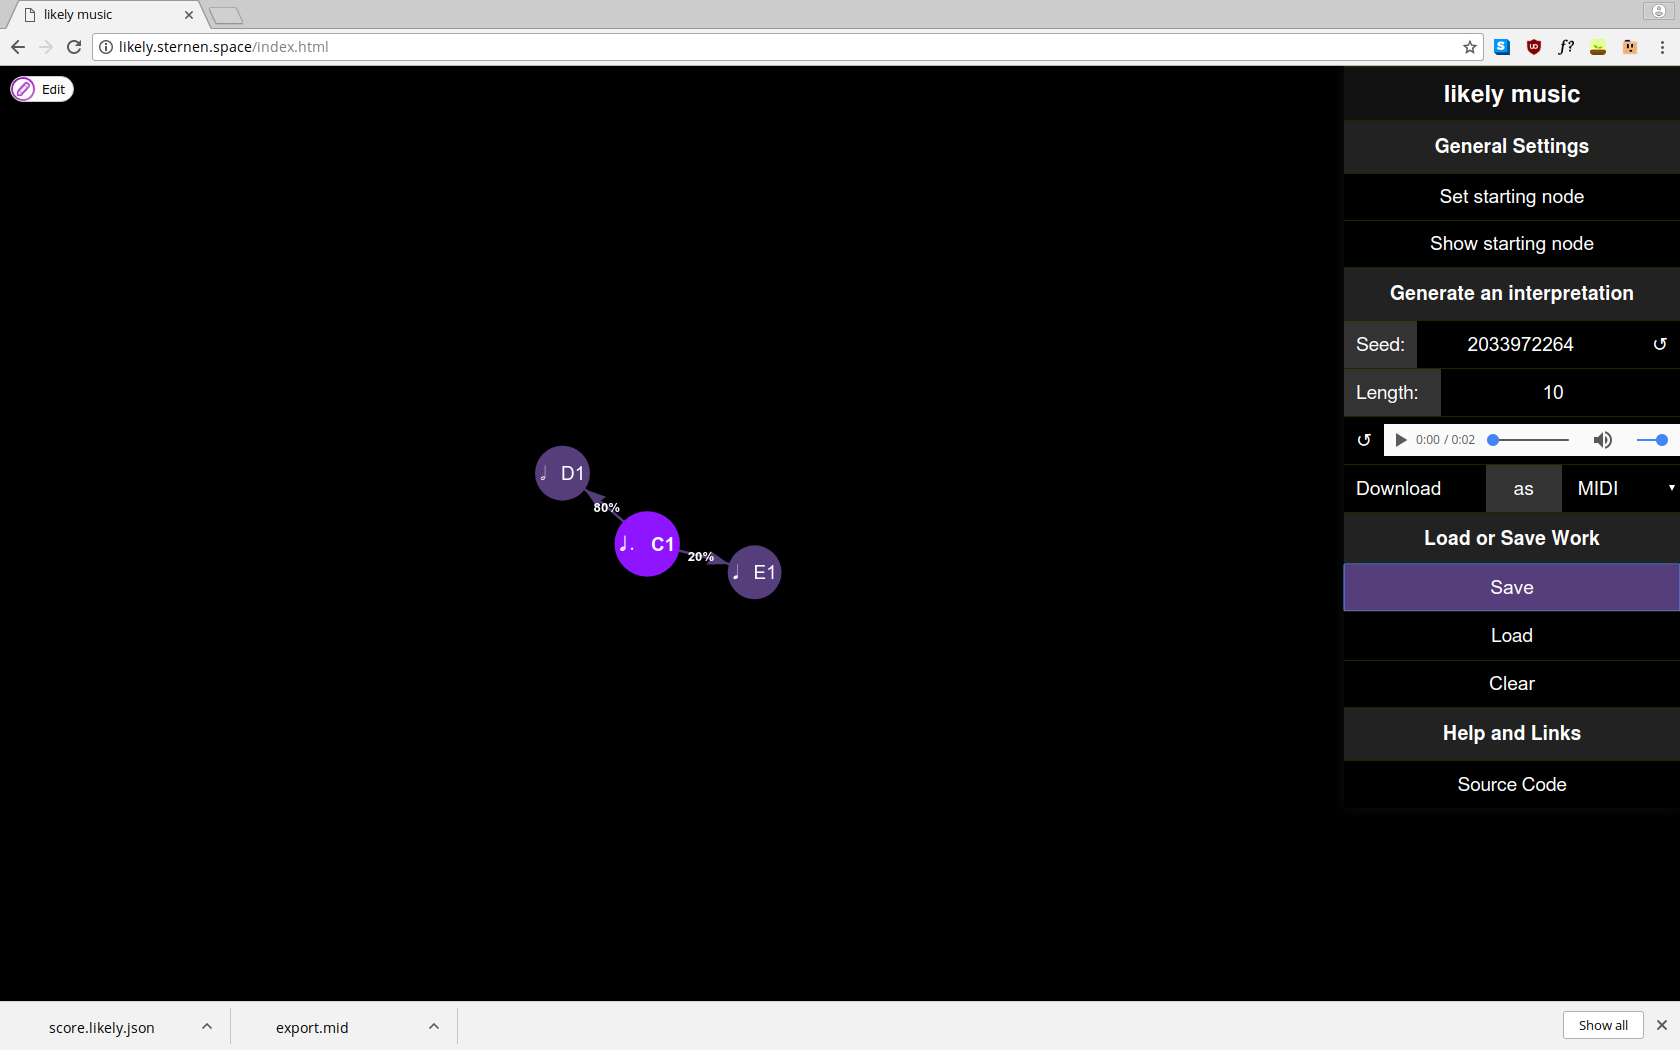
\includegraphics[width=.7\textwidth]{screenshots/save.png}
  \end{center}
  \caption{Speichern der Notation}
\end{figure}

\begin{figure}[H]
  \begin{center}
  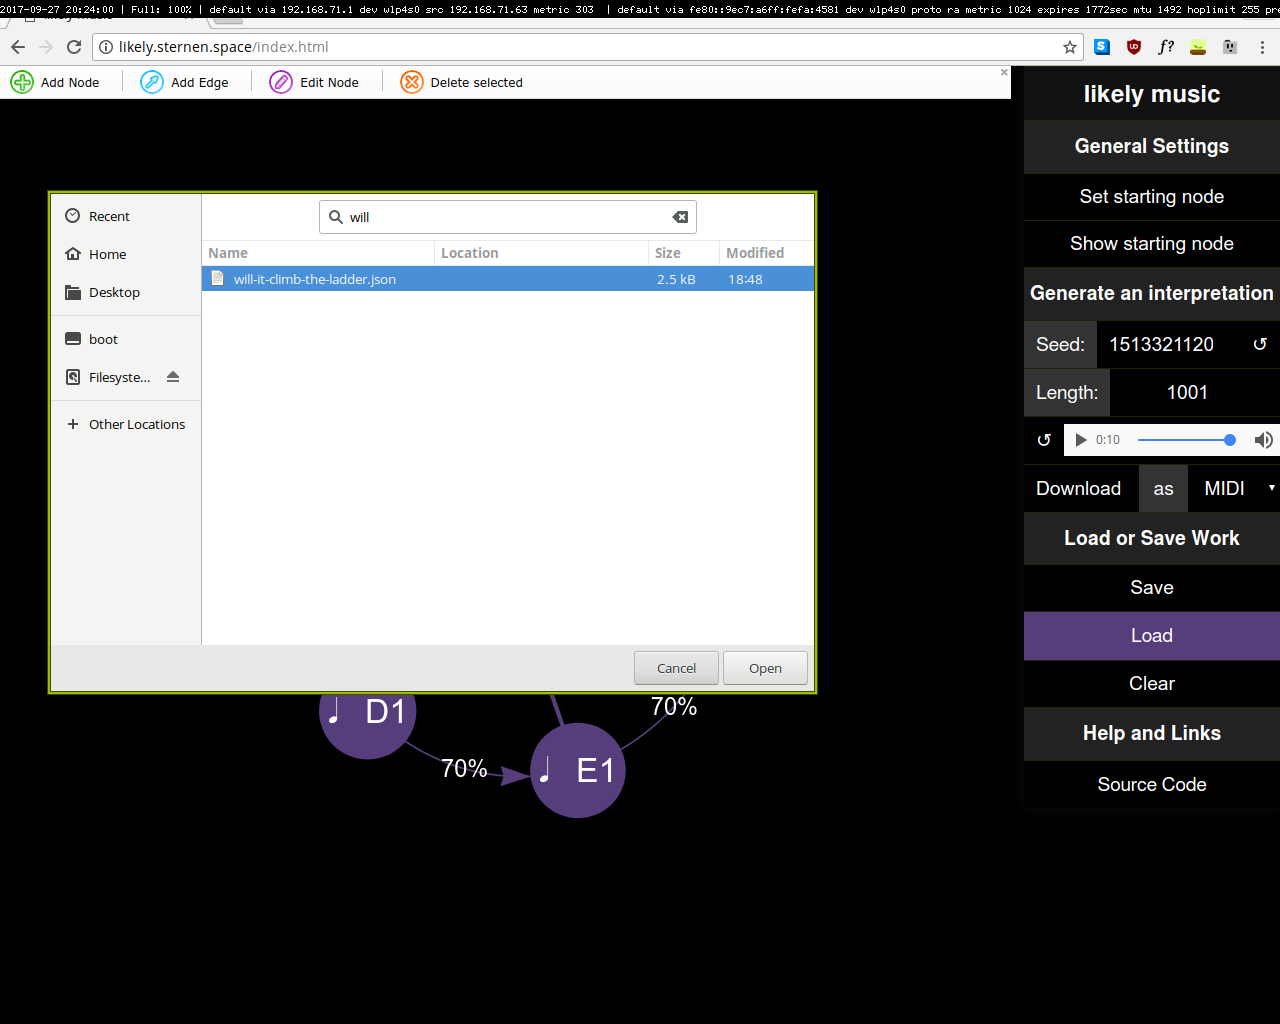
\includegraphics[width=.7\textwidth]{screenshots/load.png}
  \end{center}
  \caption{Laden einer Notation}
\end{figure}

\clearpage

\subsection*{Quelltext}
\subsubsection*{Library}
\label{sec:library}
\noindent {\bf lib/Sound/Likely.hs}
\lstinputlisting[language=haskell]{../../lib/Sound/Likely.hs}
\clearpage
\subsubsection*{Backend}
\label{sec:backend}
\noindent {\bf backend/Api.hs}
\lstinputlisting[language=haskell]{../../backend/Api.hs}
\vspace{20pt}
\noindent {\bf backend/Main.hs}
\lstinputlisting[language=haskell]{../../backend/Main.hs}
\clearpage
\subsubsection*{Web}
\label{sec:web}
\noindent {\bf web/source/index.html}
\lstinputlisting[language=html]{../../web/source/index.html}
\clearpage
\noindent {\bf web/source/custom.css}
\lstinputlisting{../../web/source/custom.css}
\clearpage
\noindent {\bf web/source/main.js}
\lstinputlisting{../../web/source/main.js}
\clearpage
\noindent {\bf Graph im JSON Format der Webapplikation}
\lstinputlisting{../../example-graph.json}

\clearpage

\subsection*{Lizenz}

\renewcommand{\abstractname}{Preamble}
\begin{abstract}
The GNU Affero General Public License is a free, copyleft license
for software and other kinds of works, specifically designed to ensure
cooperation with the community in the case of network server software.

The licenses for most software and other practical works are
designed to take away your freedom to share and change the works.  By
contrast, our General Public Licenses are intended to guarantee your
freedom to share and change all versions of a program--to make sure it
remains free software for all its users.

When we speak of free software, we are referring to freedom, not
price.  Our General Public Licenses are designed to make sure that you
have the freedom to distribute copies of free software (and charge for
them if you wish), that you receive source code or can get it if you
want it, that you can change the software or use pieces of it in new
free programs, and that you know you can do these things.

Developers that use our General Public Licenses protect your rights
with two steps: (1) assert copyright on the software, and (2) offer
you this License which gives you legal permission to copy, distribute
and/or modify the software.

A secondary benefit of defending all users' freedom is that
improvements made in alternate versions of the program, if they
receive widespread use, become available for other developers to
incorporate.  Many developers of free software are heartened and
encouraged by the resulting cooperation.  However, in the case of
software used on network servers, this result may fail to come about.
The GNU General Public License permits making a modified version and
letting the public access it on a server without ever releasing its
source code to the public.

The GNU Affero General Public License is designed specifically to
ensure that, in such cases, the modified source code becomes available
to the community.  It requires the operator of a network server to
provide the source code of the modified version running there to the
users of that server.  Therefore, public use of a modified version, on
a publicly accessible server, gives the public access to the source
code of the modified version.

An older license, called the Affero General Public License and
published by Affero, was designed to accomplish similar goals.  This is
a different license, not a version of the Affero GPL, but Affero has
released a new version of the Affero GPL which permits relicensing under
this license.

The precise terms and conditions for copying, distribution and
modification follow.
\end{abstract}

\begin{center}
{\Large \sc Terms and Conditions}
\end{center}


\begin{enumerate}

\addtocounter{enumi}{-1}

\item Definitions.

``This License'' refers to version 3 of the GNU Affero General Public License.

``Copyright'' also means copyright-like laws that apply to other kinds of
works, such as semiconductor masks.

``The Program'' refers to any copyrightable work licensed under this
License.  Each licensee is addressed as ``you''.  ``Licensees'' and
``recipients'' may be individuals or organizations.

To ``modify'' a work means to copy from or adapt all or part of the work
in a fashion requiring copyright permission, other than the making of an
exact copy.  The resulting work is called a ``modified version'' of the
earlier work or a work ``based on'' the earlier work.

A ``covered work'' means either the unmodified Program or a work based
on the Program.

To ``propagate'' a work means to do anything with it that, without
permission, would make you directly or secondarily liable for
infringement under applicable copyright law, except executing it on a
computer or modifying a private copy.  Propagation includes copying,
distribution (with or without modification), making available to the
public, and in some countries other activities as well.

To ``convey'' a work means any kind of propagation that enables other
parties to make or receive copies.  Mere interaction with a user through
a computer network, with no transfer of a copy, is not conveying.

An interactive user interface displays ``Appropriate Legal Notices''
to the extent that it includes a convenient and prominently visible
feature that (1) displays an appropriate copyright notice, and (2)
tells the user that there is no warranty for the work (except to the
extent that warranties are provided), that licensees may convey the
work under this License, and how to view a copy of this License.  If
the interface presents a list of user commands or options, such as a
menu, a prominent item in the list meets this criterion.

\item Source Code.

The ``source code'' for a work means the preferred form of the work
for making modifications to it.  ``Object code'' means any non-source
form of a work.

A ``Standard Interface'' means an interface that either is an official
standard defined by a recognized standards body, or, in the case of
interfaces specified for a particular programming language, one that
is widely used among developers working in that language.

The ``System Libraries'' of an executable work include anything, other
than the work as a whole, that (a) is included in the normal form of
packaging a Major Component, but which is not part of that Major
Component, and (b) serves only to enable use of the work with that
Major Component, or to implement a Standard Interface for which an
implementation is available to the public in source code form.  A
``Major Component'', in this context, means a major essential component
(kernel, window system, and so on) of the specific operating system
(if any) on which the executable work runs, or a compiler used to
produce the work, or an object code interpreter used to run it.

The ``Corresponding Source'' for a work in object code form means all
the source code needed to generate, install, and (for an executable
work) run the object code and to modify the work, including scripts to
control those activities.  However, it does not include the work's
System Libraries, or general-purpose tools or generally available free
programs which are used unmodified in performing those activities but
which are not part of the work.  For example, Corresponding Source
includes interface definition files associated with source files for
the work, and the source code for shared libraries and dynamically
linked subprograms that the work is specifically designed to require,
such as by intimate data communication or control flow between those
subprograms and other parts of the work.

The Corresponding Source need not include anything that users
can regenerate automatically from other parts of the Corresponding
Source.

The Corresponding Source for a work in source code form is that
same work.

\item Basic Permissions.

All rights granted under this License are granted for the term of
copyright on the Program, and are irrevocable provided the stated
conditions are met.  This License explicitly affirms your unlimited
permission to run the unmodified Program.  The output from running a
covered work is covered by this License only if the output, given its
content, constitutes a covered work.  This License acknowledges your
rights of fair use or other equivalent, as provided by copyright law.

You may make, run and propagate covered works that you do not
convey, without conditions so long as your license otherwise remains
in force.  You may convey covered works to others for the sole purpose
of having them make modifications exclusively for you, or provide you
with facilities for running those works, provided that you comply with
the terms of this License in conveying all material for which you do
not control copyright.  Those thus making or running the covered works
for you must do so exclusively on your behalf, under your direction
and control, on terms that prohibit them from making any copies of
your copyrighted material outside their relationship with you.

Conveying under any other circumstances is permitted solely under
the conditions stated below.  Sublicensing is not allowed; section 10
makes it unnecessary.

\item Protecting Users' Legal Rights From Anti-Circumvention Law.

No covered work shall be deemed part of an effective technological
measure under any applicable law fulfilling obligations under article
11 of the WIPO copyright treaty adopted on 20 December 1996, or
similar laws prohibiting or restricting circumvention of such
measures.

When you convey a covered work, you waive any legal power to forbid
circumvention of technological measures to the extent such circumvention
is effected by exercising rights under this License with respect to
the covered work, and you disclaim any intention to limit operation or
modification of the work as a means of enforcing, against the work's
users, your or third parties' legal rights to forbid circumvention of
technological measures.

\item Conveying Verbatim Copies.

You may convey verbatim copies of the Program's source code as you
receive it, in any medium, provided that you conspicuously and
appropriately publish on each copy an appropriate copyright notice;
keep intact all notices stating that this License and any
non-permissive terms added in accord with section 7 apply to the code;
keep intact all notices of the absence of any warranty; and give all
recipients a copy of this License along with the Program.

You may charge any price or no price for each copy that you convey,
and you may offer support or warranty protection for a fee.

\item Conveying Modified Source Versions.

You may convey a work based on the Program, or the modifications to
produce it from the Program, in the form of source code under the
terms of section 4, provided that you also meet all of these conditions:
  \begin{enumerate}
  \item The work must carry prominent notices stating that you modified
  it, and giving a relevant date.

  \item The work must carry prominent notices stating that it is
  released under this License and any conditions added under section
  7.  This requirement modifies the requirement in section 4 to
  ``keep intact all notices''.

  \item You must license the entire work, as a whole, under this
  License to anyone who comes into possession of a copy.  This
  License will therefore apply, along with any applicable section 7
  additional terms, to the whole of the work, and all its parts,
  regardless of how they are packaged.  This License gives no
  permission to license the work in any other way, but it does not
  invalidate such permission if you have separately received it.

  \item If the work has interactive user interfaces, each must display
  Appropriate Legal Notices; however, if the Program has interactive
  interfaces that do not display Appropriate Legal Notices, your
  work need not make them do so.
\end{enumerate}
A compilation of a covered work with other separate and independent
works, which are not by their nature extensions of the covered work,
and which are not combined with it such as to form a larger program,
in or on a volume of a storage or distribution medium, is called an
``aggregate'' if the compilation and its resulting copyright are not
used to limit the access or legal rights of the compilation's users
beyond what the individual works permit.  Inclusion of a covered work
in an aggregate does not cause this License to apply to the other
parts of the aggregate.

\item Conveying Non-Source Forms.

You may convey a covered work in object code form under the terms
of sections 4 and 5, provided that you also convey the
machine-readable Corresponding Source under the terms of this License,
in one of these ways:
  \begin{enumerate}
  \item Convey the object code in, or embodied in, a physical product
  (including a physical distribution medium), accompanied by the
  Corresponding Source fixed on a durable physical medium
  customarily used for software interchange.

  \item Convey the object code in, or embodied in, a physical product
  (including a physical distribution medium), accompanied by a
  written offer, valid for at least three years and valid for as
  long as you offer spare parts or customer support for that product
  model, to give anyone who possesses the object code either (1) a
  copy of the Corresponding Source for all the software in the
  product that is covered by this License, on a durable physical
  medium customarily used for software interchange, for a price no
  more than your reasonable cost of physically performing this
  conveying of source, or (2) access to copy the
  Corresponding Source from a network server at no charge.

  \item Convey individual copies of the object code with a copy of the
  written offer to provide the Corresponding Source.  This
  alternative is allowed only occasionally and noncommercially, and
  only if you received the object code with such an offer, in accord
  with subsection 6b.

  \item Convey the object code by offering access from a designated
  place (gratis or for a charge), and offer equivalent access to the
  Corresponding Source in the same way through the same place at no
  further charge.  You need not require recipients to copy the
  Corresponding Source along with the object code.  If the place to
  copy the object code is a network server, the Corresponding Source
  may be on a different server (operated by you or a third party)
  that supports equivalent copying facilities, provided you maintain
  clear directions next to the object code saying where to find the
  Corresponding Source.  Regardless of what server hosts the
  Corresponding Source, you remain obligated to ensure that it is
  available for as long as needed to satisfy these requirements.

  \item Convey the object code using peer-to-peer transmission, provided
  you inform other peers where the object code and Corresponding
  Source of the work are being offered to the general public at no
  charge under subsection 6d.
  \end{enumerate}

A separable portion of the object code, whose source code is excluded
from the Corresponding Source as a System Library, need not be
included in conveying the object code work.

A ``User Product'' is either (1) a ``consumer product'', which means any
tangible personal property which is normally used for personal, family,
or household purposes, or (2) anything designed or sold for incorporation
into a dwelling.  In determining whether a product is a consumer product,
doubtful cases shall be resolved in favor of coverage.  For a particular
product received by a particular user, ``normally used'' refers to a
typical or common use of that class of product, regardless of the status
of the particular user or of the way in which the particular user
actually uses, or expects or is expected to use, the product.  A product
is a consumer product regardless of whether the product has substantial
commercial, industrial or non-consumer uses, unless such uses represent
the only significant mode of use of the product.

``Installation Information'' for a User Product means any methods,
procedures, authorization keys, or other information required to install
and execute modified versions of a covered work in that User Product from
a modified version of its Corresponding Source.  The information must
suffice to ensure that the continued functioning of the modified object
code is in no case prevented or interfered with solely because
modification has been made.

If you convey an object code work under this section in, or with, or
specifically for use in, a User Product, and the conveying occurs as
part of a transaction in which the right of possession and use of the
User Product is transferred to the recipient in perpetuity or for a
fixed term (regardless of how the transaction is characterized), the
Corresponding Source conveyed under this section must be accompanied
by the Installation Information.  But this requirement does not apply
if neither you nor any third party retains the ability to install
modified object code on the User Product (for example, the work has
been installed in ROM).

The requirement to provide Installation Information does not include a
requirement to continue to provide support service, warranty, or updates
for a work that has been modified or installed by the recipient, or for
the User Product in which it has been modified or installed.  Access to a
network may be denied when the modification itself materially and
adversely affects the operation of the network or violates the rules and
protocols for communication across the network.

Corresponding Source conveyed, and Installation Information provided,
in accord with this section must be in a format that is publicly
documented (and with an implementation available to the public in
source code form), and must require no special password or key for
unpacking, reading or copying.

\item Additional Terms.

``Additional permissions'' are terms that supplement the terms of this
License by making exceptions from one or more of its conditions.
Additional permissions that are applicable to the entire Program shall
be treated as though they were included in this License, to the extent
that they are valid under applicable law.  If additional permissions
apply only to part of the Program, that part may be used separately
under those permissions, but the entire Program remains governed by
this License without regard to the additional permissions.

When you convey a copy of a covered work, you may at your option
remove any additional permissions from that copy, or from any part of
it.  (Additional permissions may be written to require their own
removal in certain cases when you modify the work.)  You may place
additional permissions on material, added by you to a covered work,
for which you have or can give appropriate copyright permission.

Notwithstanding any other provision of this License, for material you
add to a covered work, you may (if authorized by the copyright holders of
that material) supplement the terms of this License with terms:
  \begin{enumerate}
  \item Disclaiming warranty or limiting liability differently from the
  terms of sections 15 and 16 of this License; or

  \item Requiring preservation of specified reasonable legal notices or
  author attributions in that material or in the Appropriate Legal
  Notices displayed by works containing it; or

  \item Prohibiting misrepresentation of the origin of that material, or
  requiring that modified versions of such material be marked in
  reasonable ways as different from the original version; or

  \item Limiting the use for publicity purposes of names of licensors or
  authors of the material; or

  \item Declining to grant rights under trademark law for use of some
  trade names, trademarks, or service marks; or

  \item Requiring indemnification of licensors and authors of that
  material by anyone who conveys the material (or modified versions of
  it) with contractual assumptions of liability to the recipient, for
  any liability that these contractual assumptions directly impose on
  those licensors and authors.
  \end{enumerate}

All other non-permissive additional terms are considered ``further
restrictions'' within the meaning of section 10.  If the Program as you
received it, or any part of it, contains a notice stating that it is
governed by this License along with a term that is a further
restriction, you may remove that term.  If a license document contains
a further restriction but permits relicensing or conveying under this
License, you may add to a covered work material governed by the terms
of that license document, provided that the further restriction does
not survive such relicensing or conveying.

If you add terms to a covered work in accord with this section, you
must place, in the relevant source files, a statement of the
additional terms that apply to those files, or a notice indicating
where to find the applicable terms.

Additional terms, permissive or non-permissive, may be stated in the
form of a separately written license, or stated as exceptions;
the above requirements apply either way.

\item Termination.

You may not propagate or modify a covered work except as expressly
provided under this License.  Any attempt otherwise to propagate or
modify it is void, and will automatically terminate your rights under
this License (including any patent licenses granted under the third
paragraph of section 11).

However, if you cease all violation of this License, then your
license from a particular copyright holder is reinstated (a)
provisionally, unless and until the copyright holder explicitly and
finally terminates your license, and (b) permanently, if the copyright
holder fails to notify you of the violation by some reasonable means
prior to 60 days after the cessation.

Moreover, your license from a particular copyright holder is
reinstated permanently if the copyright holder notifies you of the
violation by some reasonable means, this is the first time you have
received notice of violation of this License (for any work) from that
copyright holder, and you cure the violation prior to 30 days after
your receipt of the notice.

Termination of your rights under this section does not terminate the
licenses of parties who have received copies or rights from you under
this License.  If your rights have been terminated and not permanently
reinstated, you do not qualify to receive new licenses for the same
material under section 10.

\item Acceptance Not Required for Having Copies.

You are not required to accept this License in order to receive or
run a copy of the Program.  Ancillary propagation of a covered work
occurring solely as a consequence of using peer-to-peer transmission
to receive a copy likewise does not require acceptance.  However,
nothing other than this License grants you permission to propagate or
modify any covered work.  These actions infringe copyright if you do
not accept this License.  Therefore, by modifying or propagating a
covered work, you indicate your acceptance of this License to do so.

\item Automatic Licensing of Downstream Recipients.

Each time you convey a covered work, the recipient automatically
receives a license from the original licensors, to run, modify and
propagate that work, subject to this License.  You are not responsible
for enforcing compliance by third parties with this License.

An ``entity transaction'' is a transaction transferring control of an
organization, or substantially all assets of one, or subdividing an
organization, or merging organizations.  If propagation of a covered
work results from an entity transaction, each party to that
transaction who receives a copy of the work also receives whatever
licenses to the work the party's predecessor in interest had or could
give under the previous paragraph, plus a right to possession of the
Corresponding Source of the work from the predecessor in interest, if
the predecessor has it or can get it with reasonable efforts.

You may not impose any further restrictions on the exercise of the
rights granted or affirmed under this License.  For example, you may
not impose a license fee, royalty, or other charge for exercise of
rights granted under this License, and you may not initiate litigation
(including a cross-claim or counterclaim in a lawsuit) alleging that
any patent claim is infringed by making, using, selling, offering for
sale, or importing the Program or any portion of it.

\item Patents.

A ``contributor'' is a copyright holder who authorizes use under this
License of the Program or a work on which the Program is based.  The
work thus licensed is called the contributor's ``contributor version''.

A contributor's ``essential patent claims'' are all patent claims
owned or controlled by the contributor, whether already acquired or
hereafter acquired, that would be infringed by some manner, permitted
by this License, of making, using, or selling its contributor version,
but do not include claims that would be infringed only as a
consequence of further modification of the contributor version.  For
purposes of this definition, ``control'' includes the right to grant
patent sublicenses in a manner consistent with the requirements of
this License.

Each contributor grants you a non-exclusive, worldwide, royalty-free
patent license under the contributor's essential patent claims, to
make, use, sell, offer for sale, import and otherwise run, modify and
propagate the contents of its contributor version.

In the following three paragraphs, a ``patent license'' is any express
agreement or commitment, however denominated, not to enforce a patent
(such as an express permission to practice a patent or covenant not to
sue for patent infringement).  To ``grant'' such a patent license to a
party means to make such an agreement or commitment not to enforce a
patent against the party.

If you convey a covered work, knowingly relying on a patent license,
and the Corresponding Source of the work is not available for anyone
to copy, free of charge and under the terms of this License, through a
publicly available network server or other readily accessible means,
then you must either (1) cause the Corresponding Source to be so
available, or (2) arrange to deprive yourself of the benefit of the
patent license for this particular work, or (3) arrange, in a manner
consistent with the requirements of this License, to extend the patent
license to downstream recipients.  ``Knowingly relying'' means you have
actual knowledge that, but for the patent license, your conveying the
covered work in a country, or your recipient's use of the covered work
in a country, would infringe one or more identifiable patents in that
country that you have reason to believe are valid.

If, pursuant to or in connection with a single transaction or
arrangement, you convey, or propagate by procuring conveyance of, a
covered work, and grant a patent license to some of the parties
receiving the covered work authorizing them to use, propagate, modify
or convey a specific copy of the covered work, then the patent license
you grant is automatically extended to all recipients of the covered
work and works based on it.

A patent license is ``discriminatory'' if it does not include within
the scope of its coverage, prohibits the exercise of, or is
conditioned on the non-exercise of one or more of the rights that are
specifically granted under this License.  You may not convey a covered
work if you are a party to an arrangement with a third party that is
in the business of distributing software, under which you make payment
to the third party based on the extent of your activity of conveying
the work, and under which the third party grants, to any of the
parties who would receive the covered work from you, a discriminatory
patent license (a) in connection with copies of the covered work
conveyed by you (or copies made from those copies), or (b) primarily
for and in connection with specific products or compilations that
contain the covered work, unless you entered into that arrangement,
or that patent license was granted, prior to 28 March 2007.

Nothing in this License shall be construed as excluding or limiting
any implied license or other defenses to infringement that may
otherwise be available to you under applicable patent law.

\item No Surrender of Others' Freedom.

If conditions are imposed on you (whether by court order, agreement or
otherwise) that contradict the conditions of this License, they do not
excuse you from the conditions of this License.  If you cannot convey a
covered work so as to satisfy simultaneously your obligations under this
License and any other pertinent obligations, then as a consequence you may
not convey it at all.  For example, if you agree to terms that obligate you
to collect a royalty for further conveying from those to whom you convey
the Program, the only way you could satisfy both those terms and this
License would be to refrain entirely from conveying the Program.

\item Remote Network Interaction; Use with the GNU General Public License.

Notwithstanding any other provision of this License, if you modify the
Program, your modified version must prominently offer all users interacting
with it remotely through a computer network (if your version supports such
interaction) an opportunity to receive the Corresponding Source of your
version by providing access to the Corresponding Source from a network
server at no charge, through some standard or customary means of
facilitating copying of software.  This Corresponding Source shall include
the Corresponding Source for any work covered by version 3 of the GNU
General Public License that is incorporated pursuant to the following
paragraph.

Notwithstanding any other provision of this License, you have permission to
link or combine any covered work with a work licensed under version 3 of
the GNU General Public License into a single combined work, and to convey
the resulting work.  The terms of this License will continue to apply to
the part which is the covered work, but the work with which it is combined
will remain governed by version 3 of the GNU General Public License.

\item Revised Versions of this License.

The Free Software Foundation may publish revised and/or new versions of
the GNU Affero General Public License from time to time.  Such new versions will
be similar in spirit to the present version, but may differ in detail to
address new problems or concerns.

Each version is given a distinguishing version number.  If the
Program specifies that a certain numbered version of the GNU Affero General
Public License ``or any later version'' applies to it, you have the
option of following the terms and conditions either of that numbered
version or of any later version published by the Free Software
Foundation.  If the Program does not specify a version number of the
GNU Affero General Public License, you may choose any version ever published
by the Free Software Foundation.

If the Program specifies that a proxy can decide which future
versions of the GNU Affero General Public License can be used, that proxy's
public statement of acceptance of a version permanently authorizes you
to choose that version for the Program.

Later license versions may give you additional or different
permissions.  However, no additional obligations are imposed on any
author or copyright holder as a result of your choosing to follow a
later version.

\item Disclaimer of Warranty.

\begin{sloppypar}
 THERE IS NO WARRANTY FOR THE PROGRAM, TO THE EXTENT PERMITTED BY
 APPLICABLE LAW.  EXCEPT WHEN OTHERWISE STATED IN WRITING THE
 COPYRIGHT HOLDERS AND/OR OTHER PARTIES PROVIDE THE PROGRAM ``AS IS''
 WITHOUT WARRANTY OF ANY KIND, EITHER EXPRESSED OR IMPLIED,
 INCLUDING, BUT NOT LIMITED TO, THE IMPLIED WARRANTIES OF
 MERCHANTABILITY AND FITNESS FOR A PARTICULAR PURPOSE.  THE ENTIRE
 RISK AS TO THE QUALITY AND PERFORMANCE OF THE PROGRAM IS WITH YOU.
 SHOULD THE PROGRAM PROVE DEFECTIVE, YOU ASSUME THE COST OF ALL
 NECESSARY SERVICING, REPAIR OR CORRECTION.
\end{sloppypar}

\item Limitation of Liability.

 IN NO EVENT UNLESS REQUIRED BY APPLICABLE LAW OR AGREED TO IN
 WRITING WILL ANY COPYRIGHT HOLDER, OR ANY OTHER PARTY WHO MODIFIES
 AND/OR CONVEYS THE PROGRAM AS PERMITTED ABOVE, BE LIABLE TO YOU FOR
 DAMAGES, INCLUDING ANY GENERAL, SPECIAL, INCIDENTAL OR CONSEQUENTIAL
 DAMAGES ARISING OUT OF THE USE OR INABILITY TO USE THE PROGRAM
 (INCLUDING BUT NOT LIMITED TO LOSS OF DATA OR DATA BEING RENDERED
 INACCURATE OR LOSSES SUSTAINED BY YOU OR THIRD PARTIES OR A FAILURE
 OF THE PROGRAM TO OPERATE WITH ANY OTHER PROGRAMS), EVEN IF SUCH
 HOLDER OR OTHER PARTY HAS BEEN ADVISED OF THE POSSIBILITY OF SUCH
 DAMAGES.

\item Interpretation of Sections 15 and 16.

If the disclaimer of warranty and limitation of liability provided
above cannot be given local legal effect according to their terms,
reviewing courts shall apply local law that most closely approximates
an absolute waiver of all civil liability in connection with the
Program, unless a warranty or assumption of liability accompanies a
copy of the Program in return for a fee.

\begin{center}
{\Large\sc End of Terms and Conditions}

\bigskip
How to Apply These Terms to Your New Programs
\end{center}

If you develop a new program, and you want it to be of the greatest
possible use to the public, the best way to achieve this is to make it
free software which everyone can redistribute and change under these terms.

To do so, attach the following notices to the program.  It is safest
to attach them to the start of each source file to most effectively
state the exclusion of warranty; and each file should have at least
the ``copyright'' line and a pointer to where the full notice is found.

{\footnotesize
\begin{verbatim}
<one line to give the program's name and a brief idea of what it does.>

Copyright (C) <textyear>  <name of author>

This program is free software: you can redistribute it and/or modify
it under the terms of the GNU Affero General Public License as published by
the Free Software Foundation, either version 3 of the License, or
(at your option) any later version.

This program is distributed in the hope that it will be useful,
but WITHOUT ANY WARRANTY; without even the implied warranty of
MERCHANTABILITY or FITNESS FOR A PARTICULAR PURPOSE.  See the
GNU Affero General Public License for more details.

You should have received a copy of the GNU Affero General Public License
along with this program.  If not, see <http://www.gnu.org/licenses/>.
\end{verbatim}
}

Also add information on how to contact you by electronic and paper mail.

If your software can interact with users remotely through a computer
network, you should also make sure that it provides a way for users to
get its source.  For example, if your program is a web application, its
interface could display a ``Source'' link that leads users to an archive
of the code.  There are many ways you could offer source, and different
solutions will be better for different programs; see section 13 for the
specific requirements.

You should also get your employer (if you work as a programmer) or
school, if any, to sign a ``copyright disclaimer'' for the program, if
necessary.  For more information on this, and how to apply and follow
the GNU AGPL, see \texttt{http://www.gnu.org/licenses/}.

\end{enumerate}

\end{document}
